\documentclass{beamer}

%\usepackage[utf8]{inputenc}
%\usetheme{Frankfurt}
\usetheme{Rochester}
\setbeamercovered{transparent}
\usepackage{dsfont}
%\usepackage[pdftex]{graphicx}
\usepackage{graphicx}
%\usepackage[noline,noend,ruled]{algorithm2e}
%\renewcommand{\algorithmcfname}{ALGORITHM}
\usepackage{amsfonts}
\usepackage{amsmath}
\usepackage{amssymb}
\usepackage{wasysym}
\usepackage{cclicenses}
\usepackage{listings}
\usepackage{xcolor}
%\usepackage[all]{xy}
%\usepackage{pifont}



\title{Measuring Icebergs @CoronaSurveys}
\author{Davide Frey \& @CoronaSurveys Team\\
\vspace{8pt}WIDE Team, Inria Rennes}
\date{4 May 2020}

\begin{document}

\frame[plain]{
\titlepage
\begin{center}
%
\includegraphics[width=0.33\textwidth]{inesctec.jpg}\\
%
\includegraphics[width=0.33\textwidth]{UMinho.png}
%\includegraphics[width=0.3\textwidth]{INESCTECcomb_VPH_EN_CP_rgb.jpg}
\end{center}
}

% \begin{frame}

  % \frametitle{Spain, March 13th 2020}
%   \begin{itemize}
%     \item El País ``Spain is the second EU country in number of cases''

%     \item Reuters ``The Spanish health ministry said the number of coronavirus cases in the country jumped to 4,209 on Friday from Thursday's 3,004 as the disease spread mostly in Madrid, the Basque Country and La Rioja regions.''
% %The death toll from the coronavirus epidemic in the country has increased to 120 from 84 the previous day.
%   \end{itemize}
% \vspace{1ex}
%   Rapid growth: hard to keep up with testing and reporting delays. \\
%   \vspace{3ex}
%   Not only in Spain, but also in France, Italy, and most countries.

% \end{frame}

\begin{frame}
  \frametitle{Spain, March 13th 2020}
  \framesubtitle{Antonio Fernandez Anta, IMDEA Networks, Spain}
  \begin{center}
  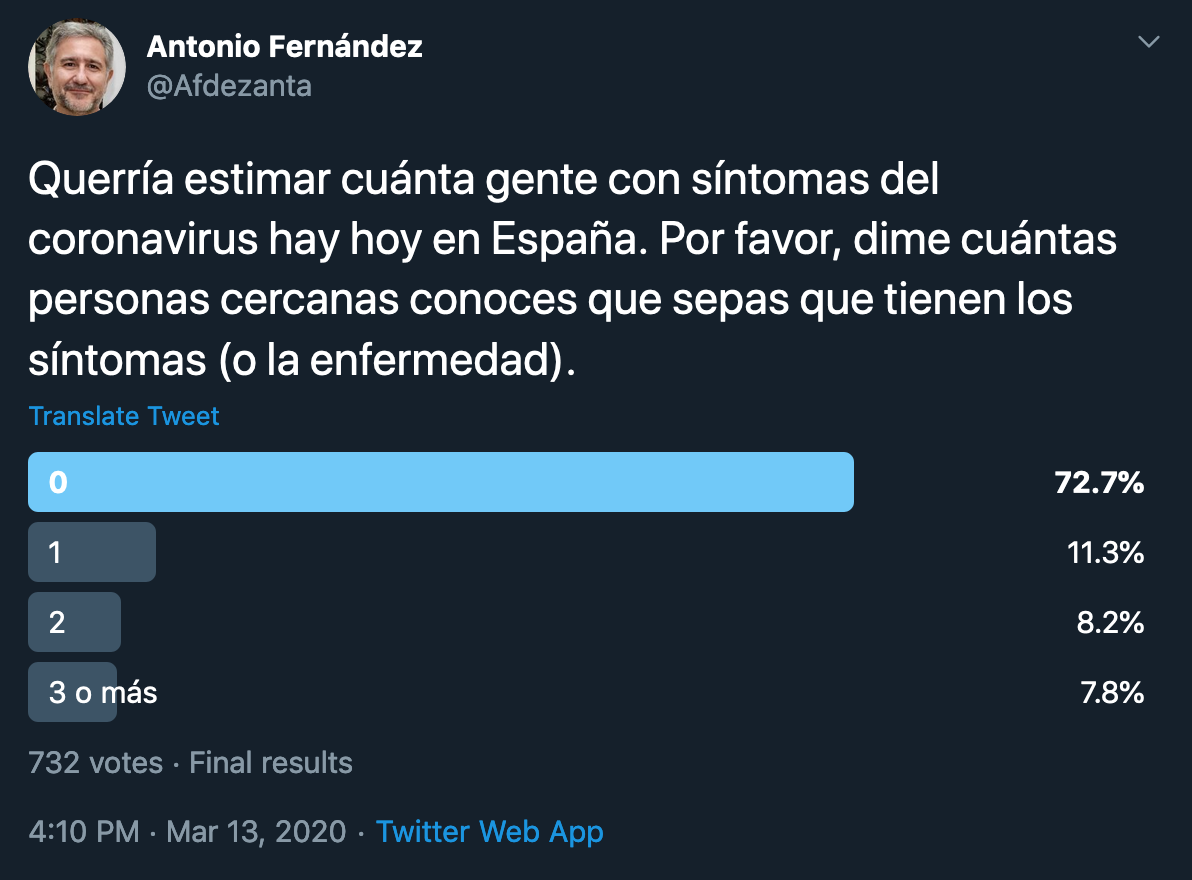
\includegraphics[width=0.5\textwidth]{Twitter.png}
  \end{center}
  \begin{itemize}
    \item $\textit{cases}=374$, $\textit{reach}=732*150$ \hfill (Dunbar number is 150)
    \item $\textit{total}=\frac{\textit{cases}}{\textit{reach}}*\textit{ESpop} \approx 153000 $ \hfill ($\approx 30*$ official)
  \end{itemize}
\end{frame}

\begin{frame}
\frametitle{From Twitter to Google Forms}
\begin{itemize}
\item Spread the survey beyond Spain 
\item Initial countries:\\
Spain, Italy, Portugal, UK, USA, Germany, Cyprus 
\item French Survey Timeline
\begin{itemize}
\item March 20: Antonio Fernandez contacted me and several other researchers
\item March 22: First ``daily'' survey in France on Google Forms
\item March 23-27: COERLE's  feedback
\item March 28-today: Survey Resumes: Google Forms, always open. 
\end{itemize}
\item Currently 24 countries + Arab countries + rest of the world
\item Migrating survey off Google Forms. 
\end{itemize}
\end{frame}

\begin{frame}
  \frametitle{Two ``simple'' questions}
  For any given country/region and after informed consent we ask:
  \begin{center}
  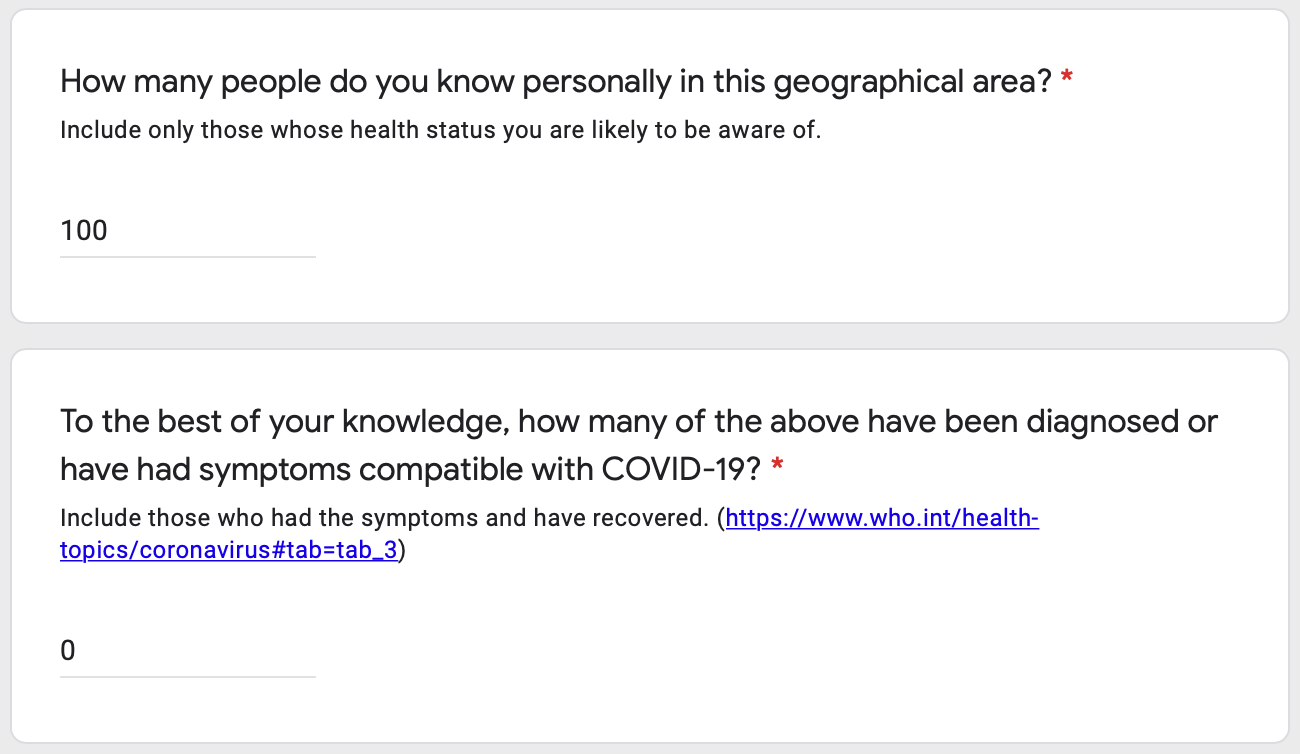
\includegraphics[width=0.75\textwidth]{Questions.png}
  \end{center}
  A few optional questions to be added in new version
  \begin{itemize}
  \item estimate network bias, and other parameters 
  \item without collecting personal information
  \end{itemize}

\end{frame}



\begin{frame}
  \frametitle{Trade-offs in Open Surveys}

 Positive Points:
  \begin{itemize}
    \item No personal data: health status of respondent is not asked
    \item No GDPR issues \hfill (but Ethical Board approval)
    \item Number of answers and reach size
  \end{itemize}
 Negative Points: 
  \begin{itemize}
    \item Unorthodox approach: no panel selection, no stratification
    \item Not possible to track answers from users across time
    \item Fault injections
  \end{itemize}
\end{frame}

 % (overlap)
 %  \item estimate other parameters (ICU rate, death rate, $R_0$, ...)
 %    in some countries
\begin{frame}
  \frametitle{@CoronaSurveys at https://coronasurveys.org}
  https://www.instagram.com/coronasurveys/\\
  https://tinyurl.com/coronasurveysfrance\\
  \begin{center}
  
\includegraphics[width=0.8\textwidth]{CoronaSurveys.png}
  \end{center}
\end{frame}

\begin{frame}
\frametitle{Media Presence}
\begin{center}
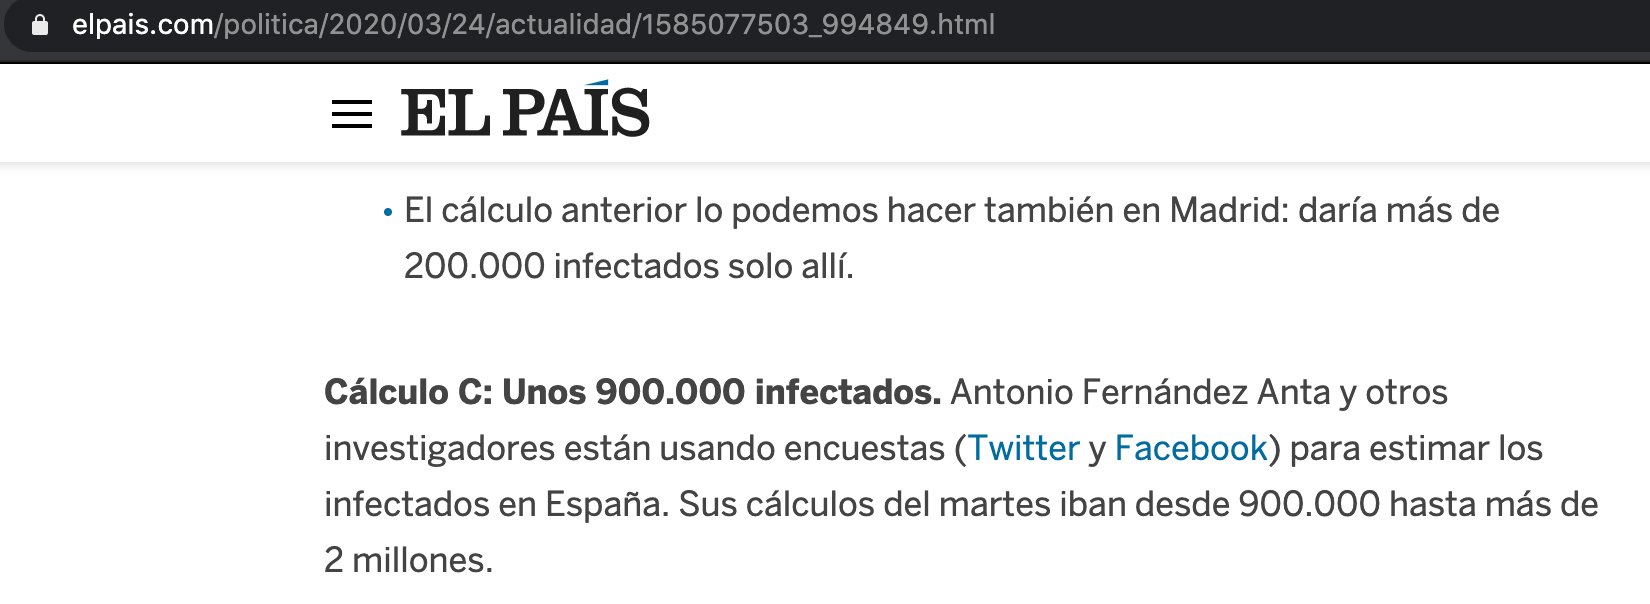
\includegraphics[width=0.7\textwidth]{elpais.png}

\includegraphics[width=0.7\textwidth]{publico.png}
\end{center}
\end{frame}
\begin{frame}
  \frametitle{Responses: Spain}
  \begin{center}
  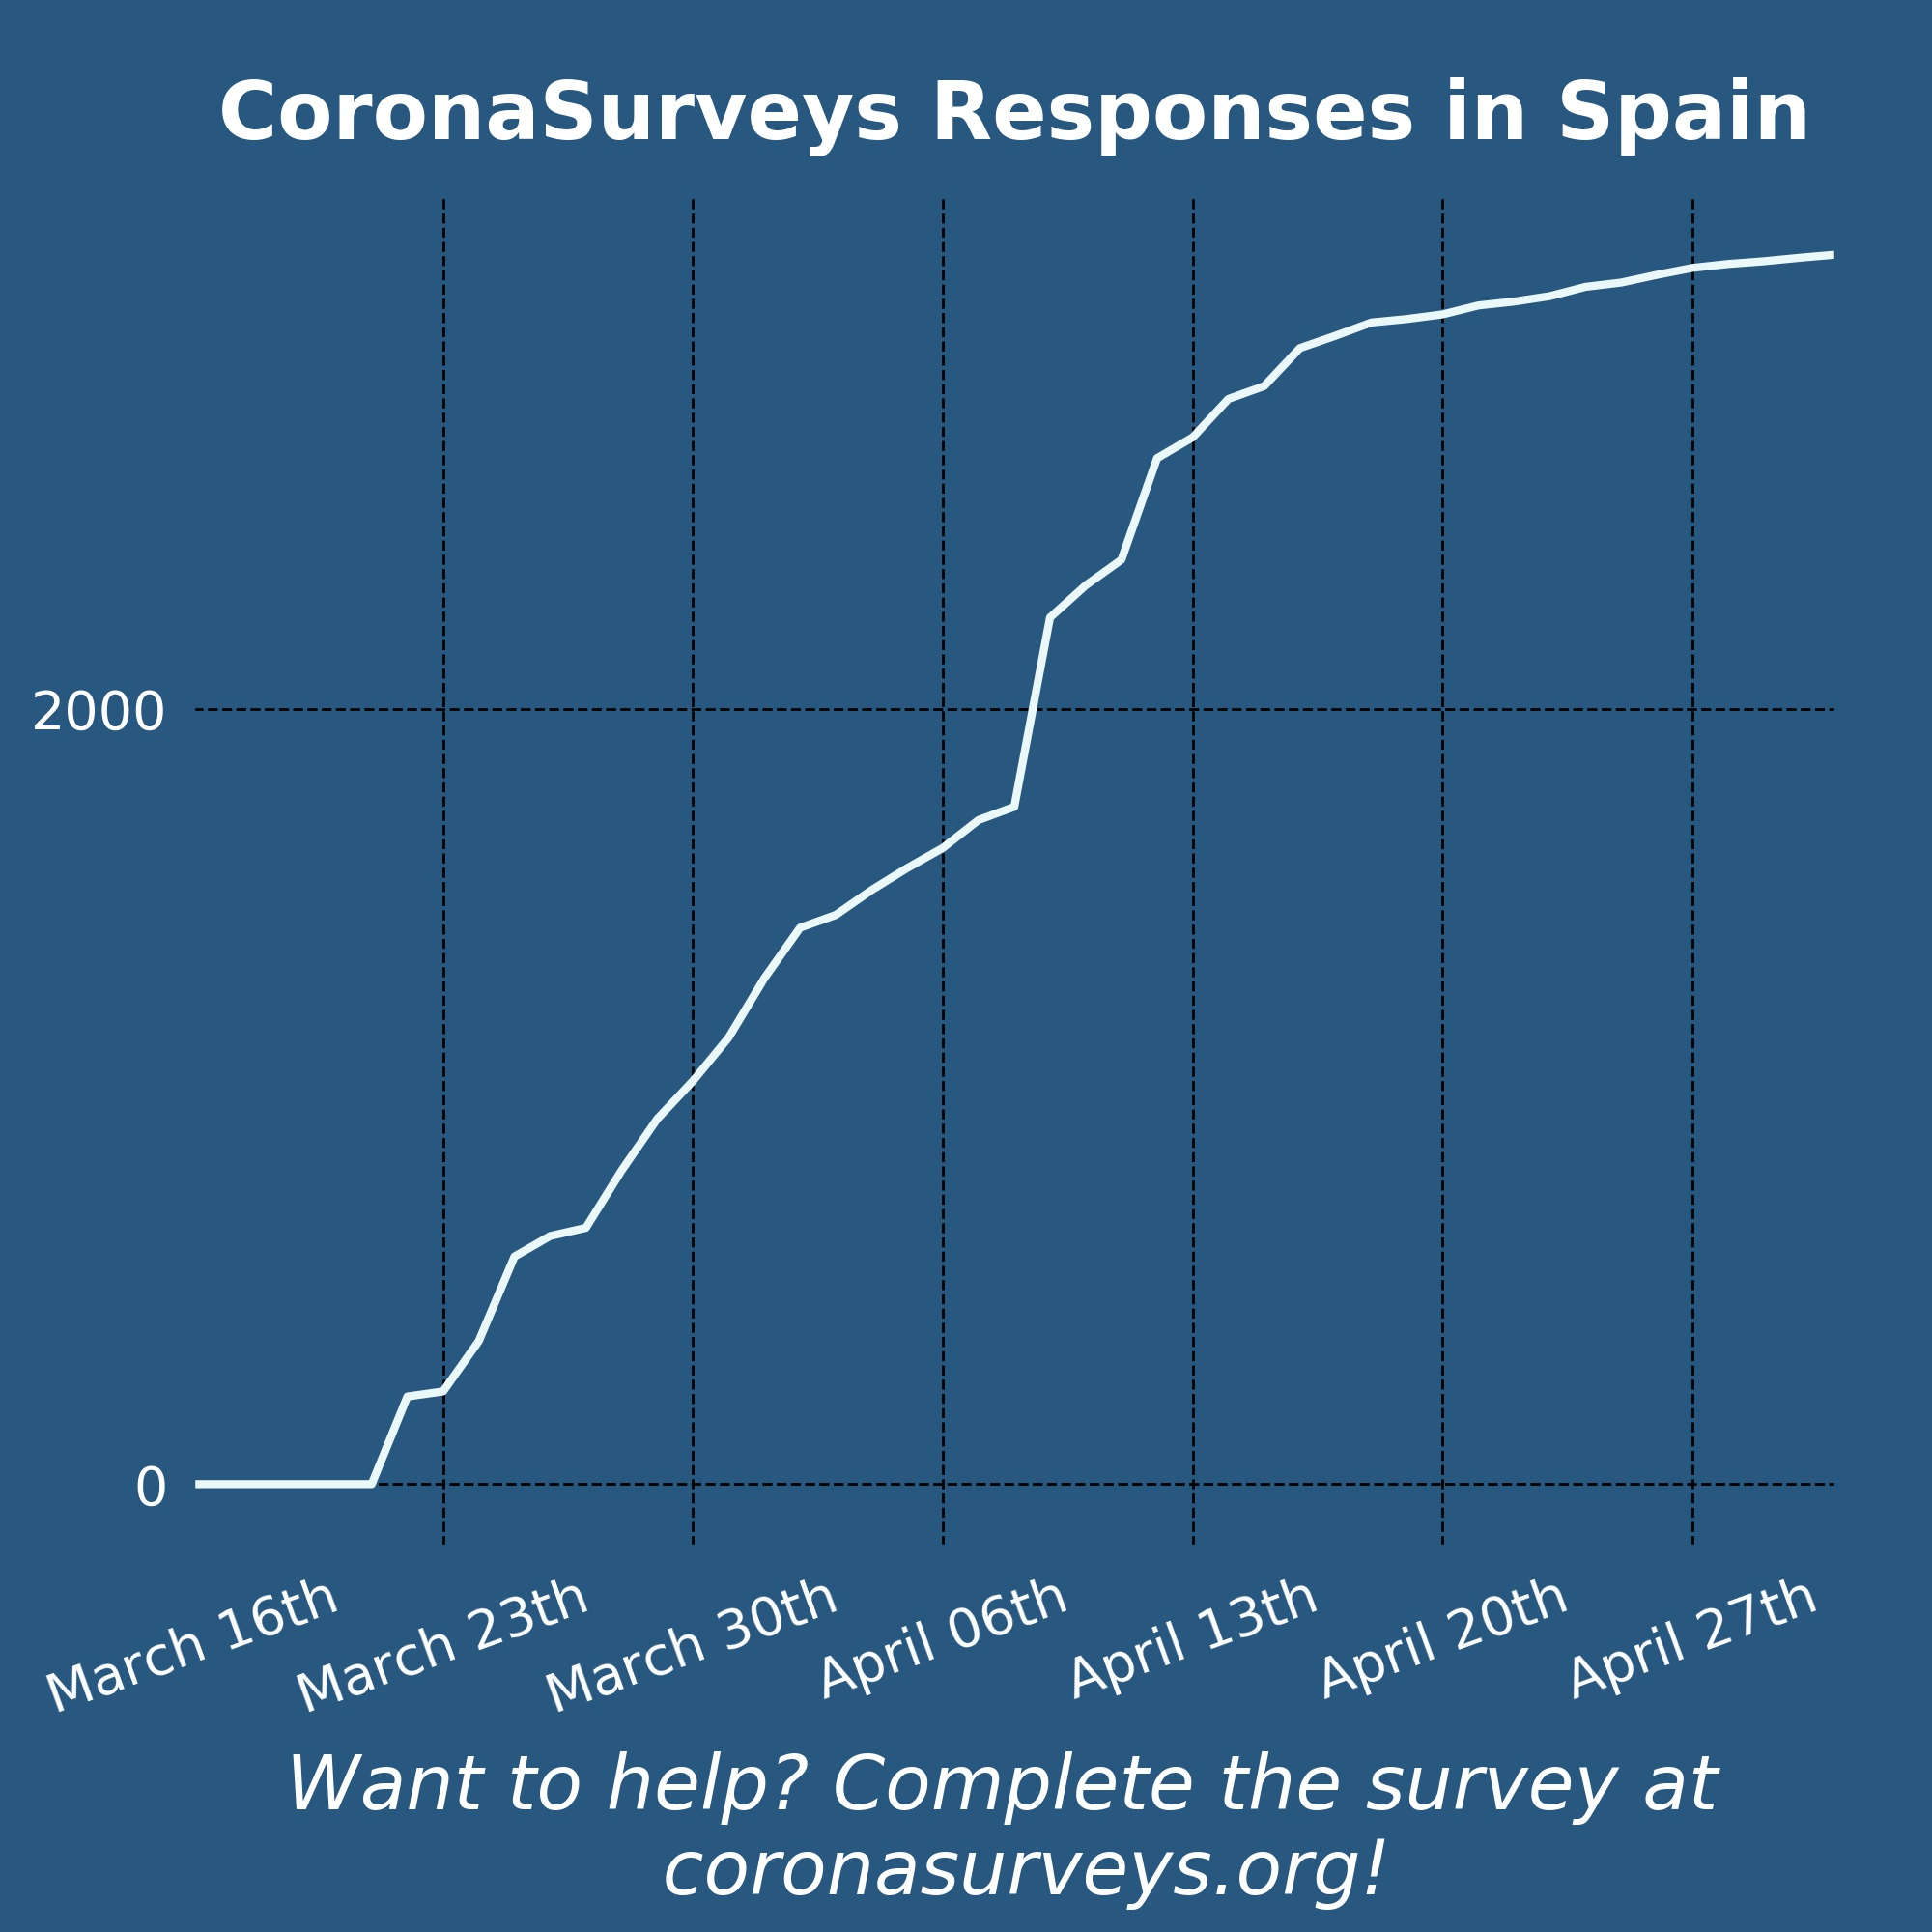
\includegraphics[width=0.7\textwidth]{responses-ES.jpg}
  \end{center}
\end{frame}

\begin{frame}
  \frametitle{Responses: Portugal}
  \begin{center}
  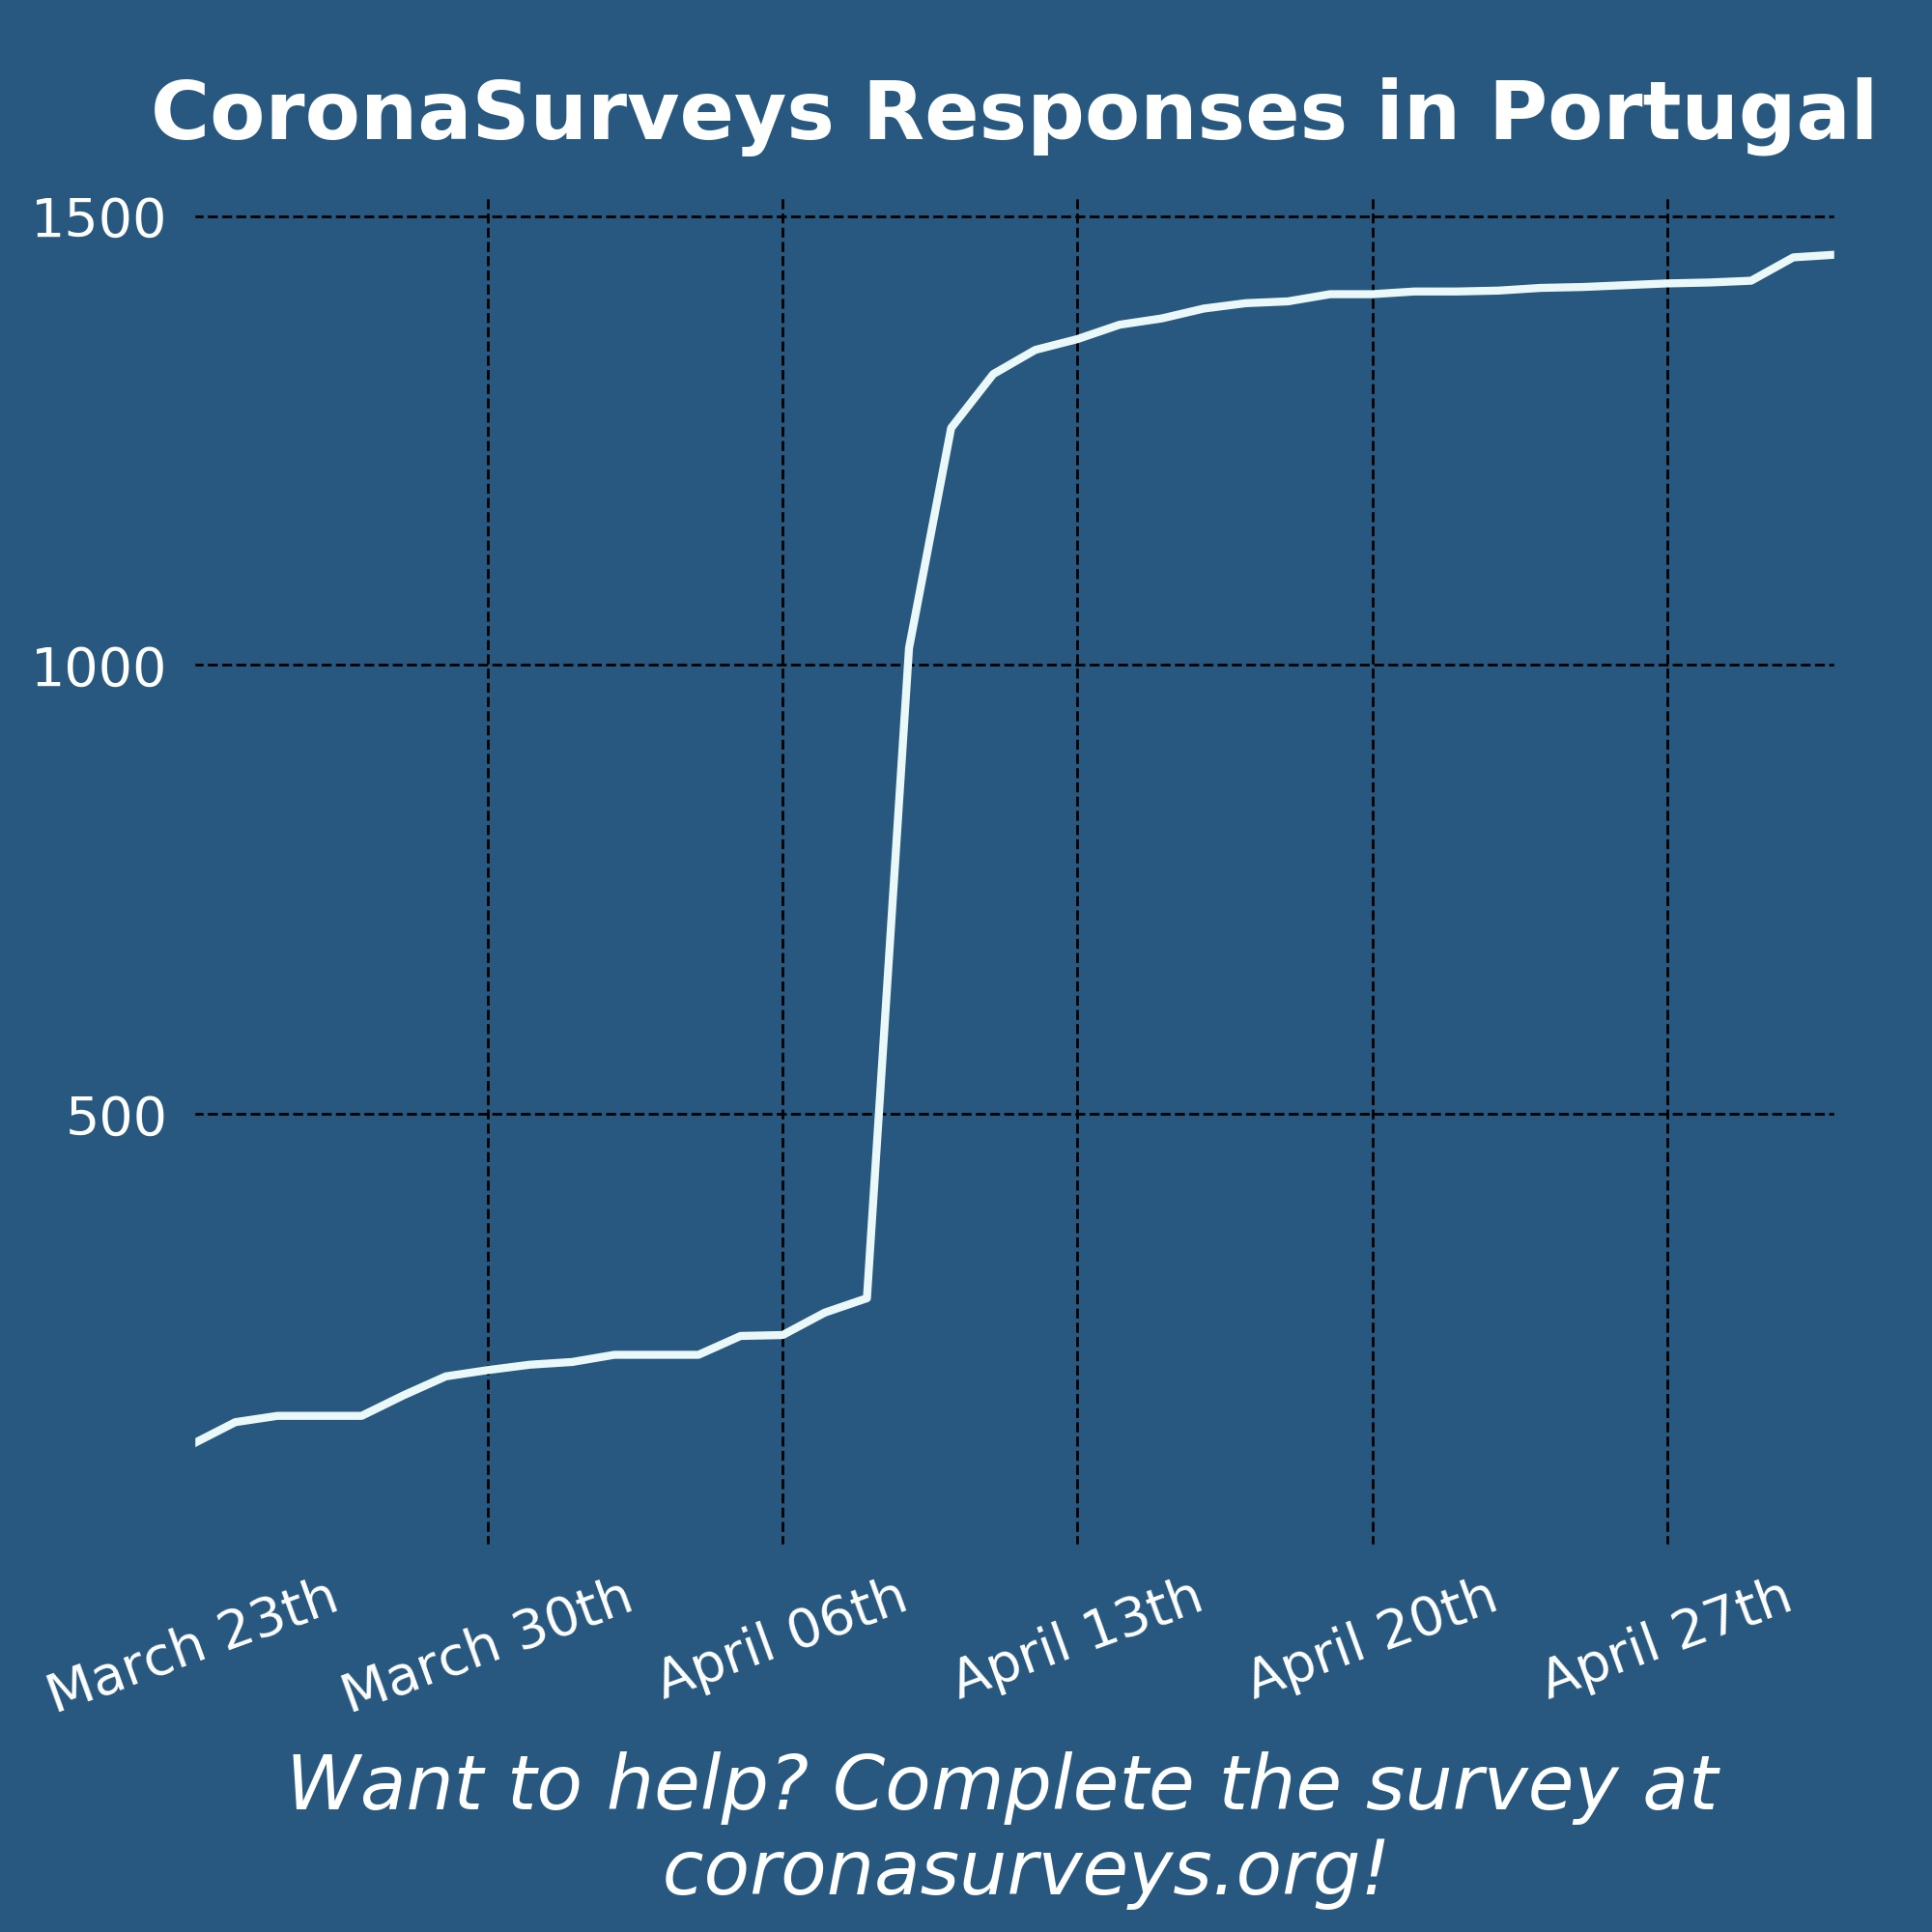
\includegraphics[width=0.7\textwidth]{responses-PT.jpg}
  \end{center}
\end{frame}


\begin{frame}
  \frametitle{Responses: France}
  \begin{center}
  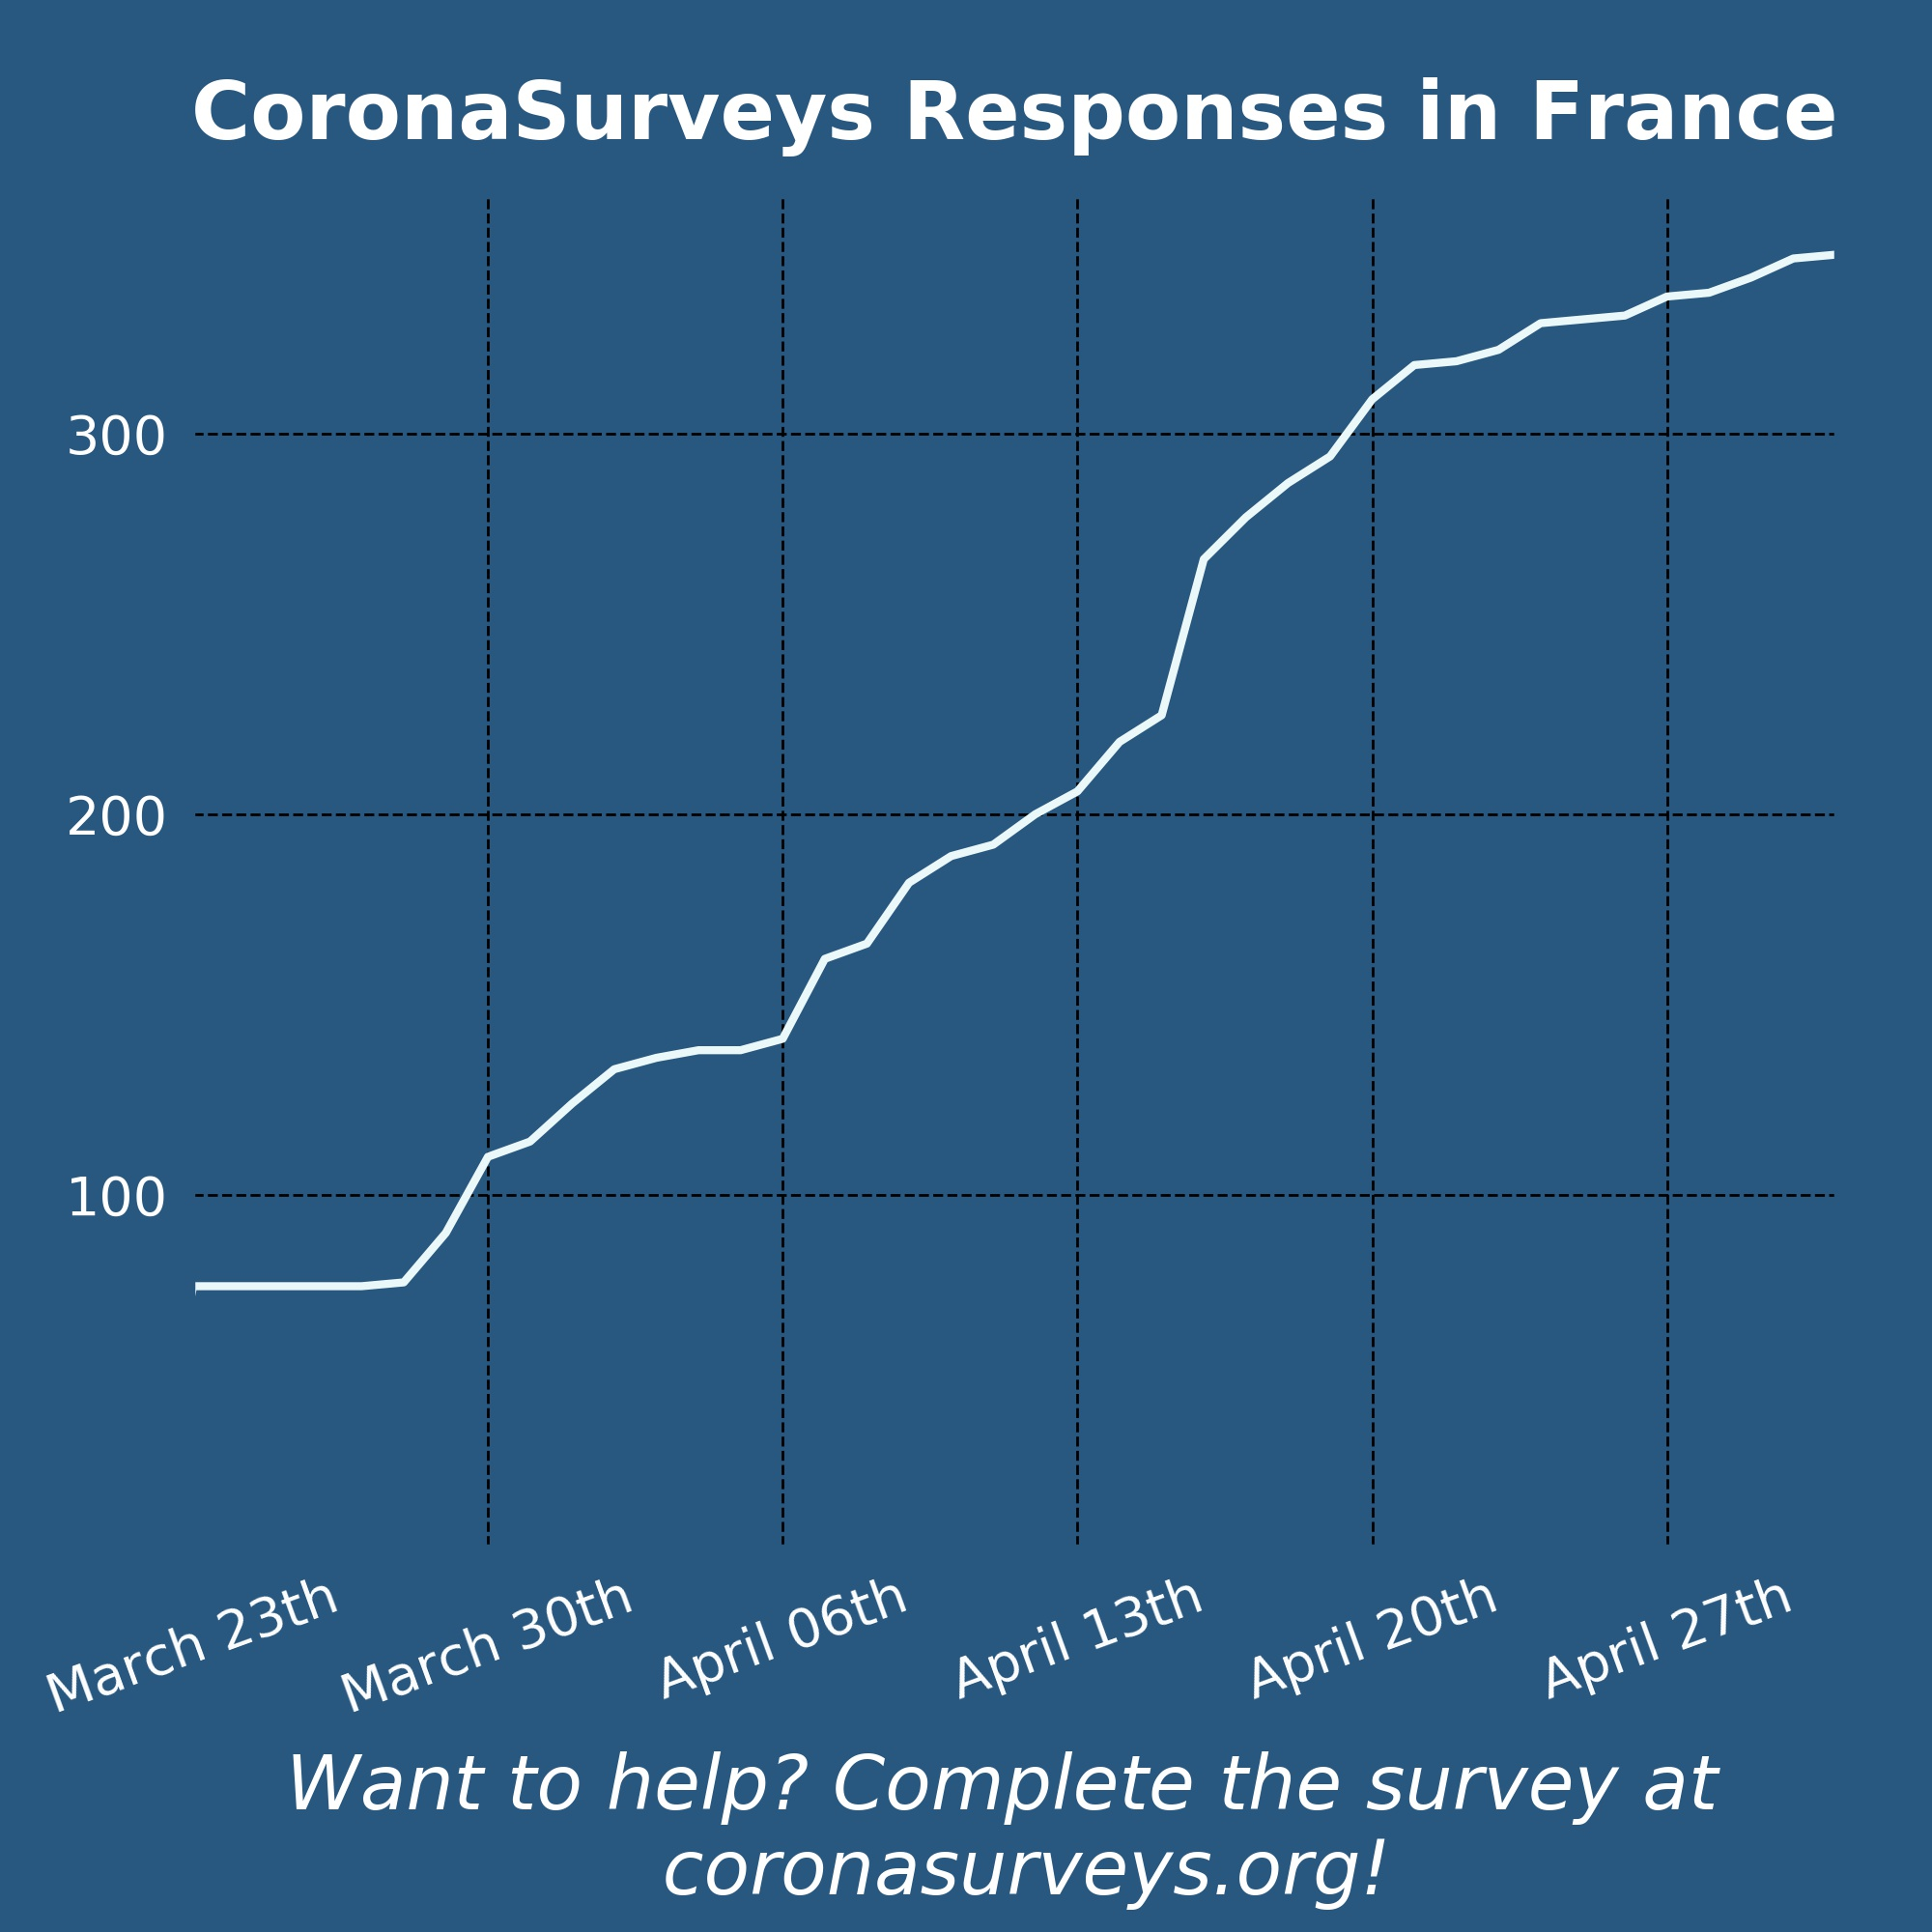
\includegraphics[width=0.7\textwidth]{responses-FR.jpg}
  \end{center}
\end{frame}

\begin{frame}
  \frametitle{Data cleaning}
  Survey responses, pairs  $(\textit{cases}_i,\textit{reach}_i)$, are cleaned by identifying and removing outliers: 
  \begin{itemize}
    \item $\textit{reach}_i$ \--- remove entries above $1.5 *$  the  interquartile  range
    \item $\frac{\textit{cases}_i}{\textit{reach}_i} < 0.3$ \--- remove entries with very high incidence
  % \end{itemize}
  % \begin{itemize}
    \item Several datapoints, from batches of 30 or more answers  
%    \item Consistent evolution across time
  \end{itemize} 



\end{frame}

\begin{frame}
  \frametitle{Estimators}
  Assume $n$ response pairs $(\textit{cases}_i,\textit{reach}_i)$, region of population $P$  

  We can produce three estimators: 
  \begin{description}
    \item[Weighted] $E_w  =  P \cdot \frac{\sum_{i} \textit{cases}_i}{\sum_{i} \textit{reach}_i}$  
    \item[Mean] $E_m  =  P \cdot \frac{\sum_i (\textit{cases}_i / \textit{reach}_i)}{n}$
    \item[Dunbar] $E_d  =  P \cdot \frac{\sum_{i} \textit{cases}_i}{n \cdot 150}$
  \end{description}
  Only showing  Weighted in the following. 


  \begin{itemize}
    \item Still, how can we know the data is meaningful?   
    \item We need other independent estimates 
  \end{itemize}


\end{frame}



\begin{frame}
  \frametitle{Fatality based estimates}
  \framesubtitle{Coarse grained: deaths * 400 estimate}
  Amy Maxmen. How much is coronavirus spreading under radar? 
  Nature News Explainer, March 13th, 2020. https://www.nature.com/articles/d41586-020-00760-8

  \begin{block}{Current deaths times 400}
  \begin{center}
  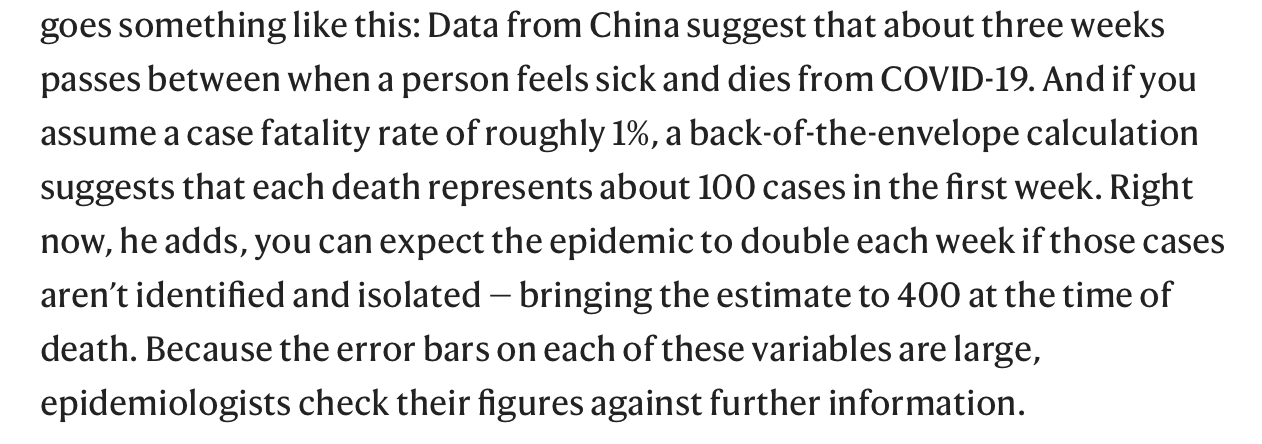
\includegraphics[width=0.9\textwidth]{Amy.png}
  \end{center}
  \end{block}
  Coarse grained estimate, only in the initial exponential growth. 
\end{frame}

\begin{frame}
  \frametitle{Fatality based estimates}
  \framesubtitle{Fine grained: cCFR estimate}
  \begin{itemize}
    \item Corrected Case Fatality Ratio $\approx$ fatalities over detected cases with known outcomes (about 2 weeks lag)
      \begin{itemize}
      \item \url{https://cmmid.github.io/topics/covid19/global_cfr_estimates.html}
      \end{itemize}

    \item Find a ``stable'' baseline for the cCFR 
      \begin{itemize}
        \item China, Wuhan, $cCFR=1.38$.  Verity et al. Lancet paper
      \end{itemize}
  \end{itemize}
\end{frame}

\begin{frame}
  \frametitle{Fatality based estimates}
  \framesubtitle{Fine grained: cCFR estimate}
  \begin{itemize}
    \item Corrected Case Fatality Ratio $\approx$ fatalities over detected cases with known outcomes (about 2 weeks lag)
    \item Find a ``stable'' baseline for the cCFR 
      \begin{itemize}
        \item China, Wuhan, $cCFR=1.38$.  Verity et al. Lancet Paper 
          \begin{block}{April 17th, Wall Street Journal}
          \begin{center}
          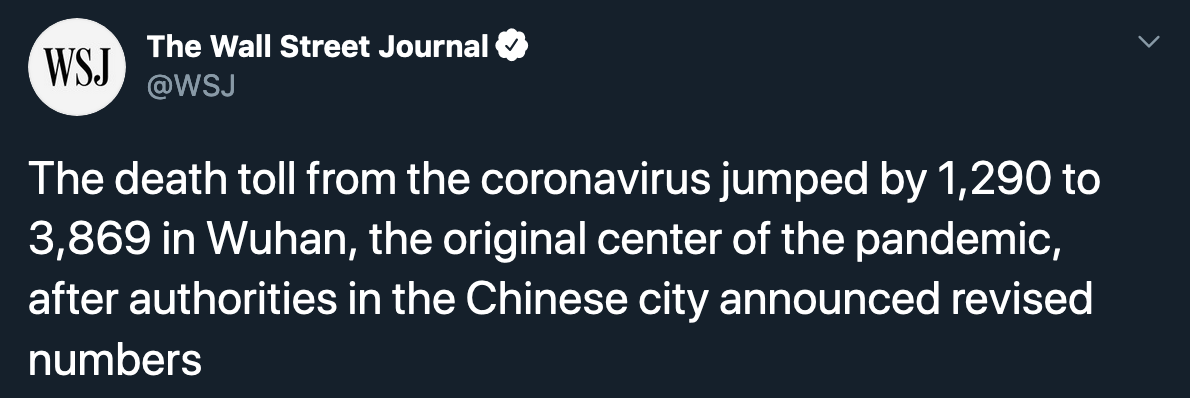
\includegraphics[width=0.9\textwidth]{WSJ.png}
          \end{center}
          \end{block}
      \end{itemize}
  \end{itemize}
\end{frame}

\begin{frame}
  \frametitle{Fatality based estimates}
  \framesubtitle{Fine grained: cCFR estimate}
  \begin{itemize}
    \item Corrected Case Fatality Ratio $\approx$ fatalities over detected cases with known outcomes (about 2 weeks lag)
    \item Find a ``stable'' baseline for the cCFR 
      \begin{itemize}
        \item China, Wuhan, $cCFR=1.38$.  Verity et al. Lancet Paper 
        \item Alternatives: Korean data, Germany Gangelt data
      \end{itemize}
    \item Calculate a country cCFR from daily ECDC data 
    \item Use proportion to baseline to infer current cases estimate
  \end{itemize} \pause

  Caveats: Baseline quality, death reporting policies, cases coverage, calibration of symptoms to death delay, missing date of symptoms.
\end{frame}

\begin{frame}
\frametitle{Summary of Estimators}
\begin{itemize}
\item Official number of cases
\item CCFR estimate
\item Coronasurveys estimate
\end{itemize}
\end{frame}

\begin{frame}
  \frametitle{Estimates, Portugal}
  \begin{center}
  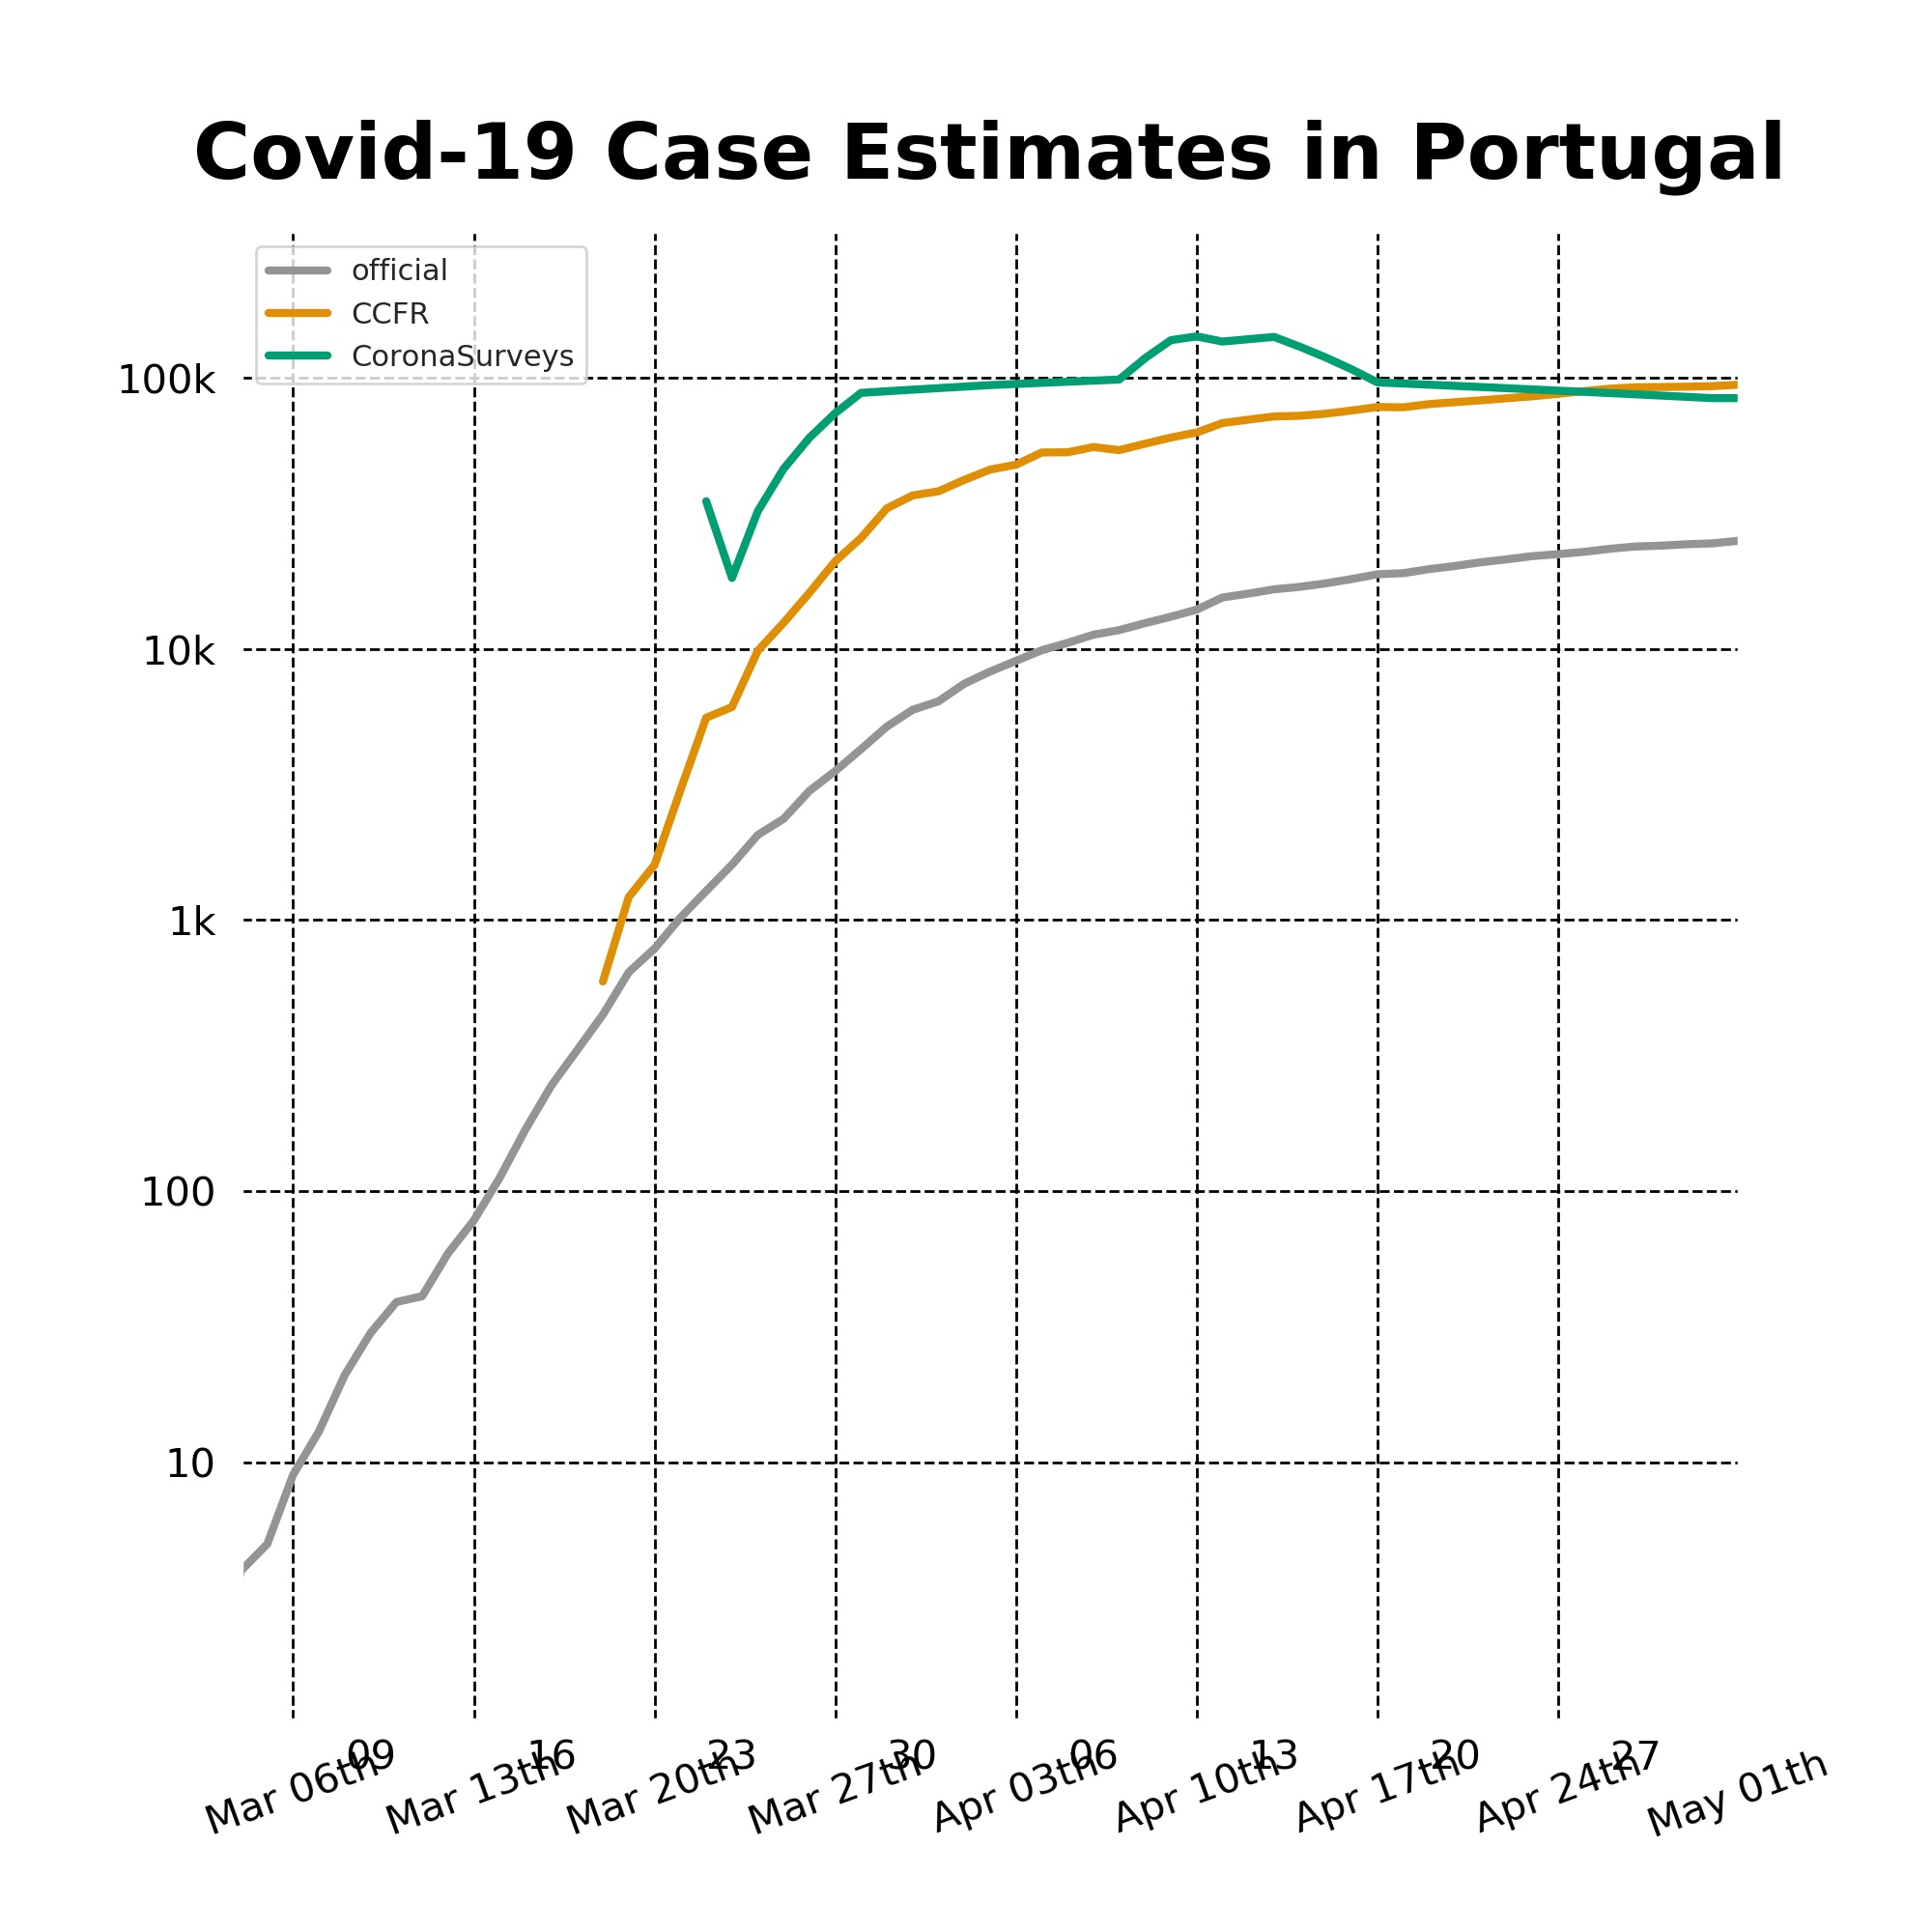
\includegraphics[width=0.7\textwidth]{estimatesPT.jpg}
  \end{center}
\end{frame}

\begin{frame}
  \frametitle{Estimates, Spain}
  \begin{center}
  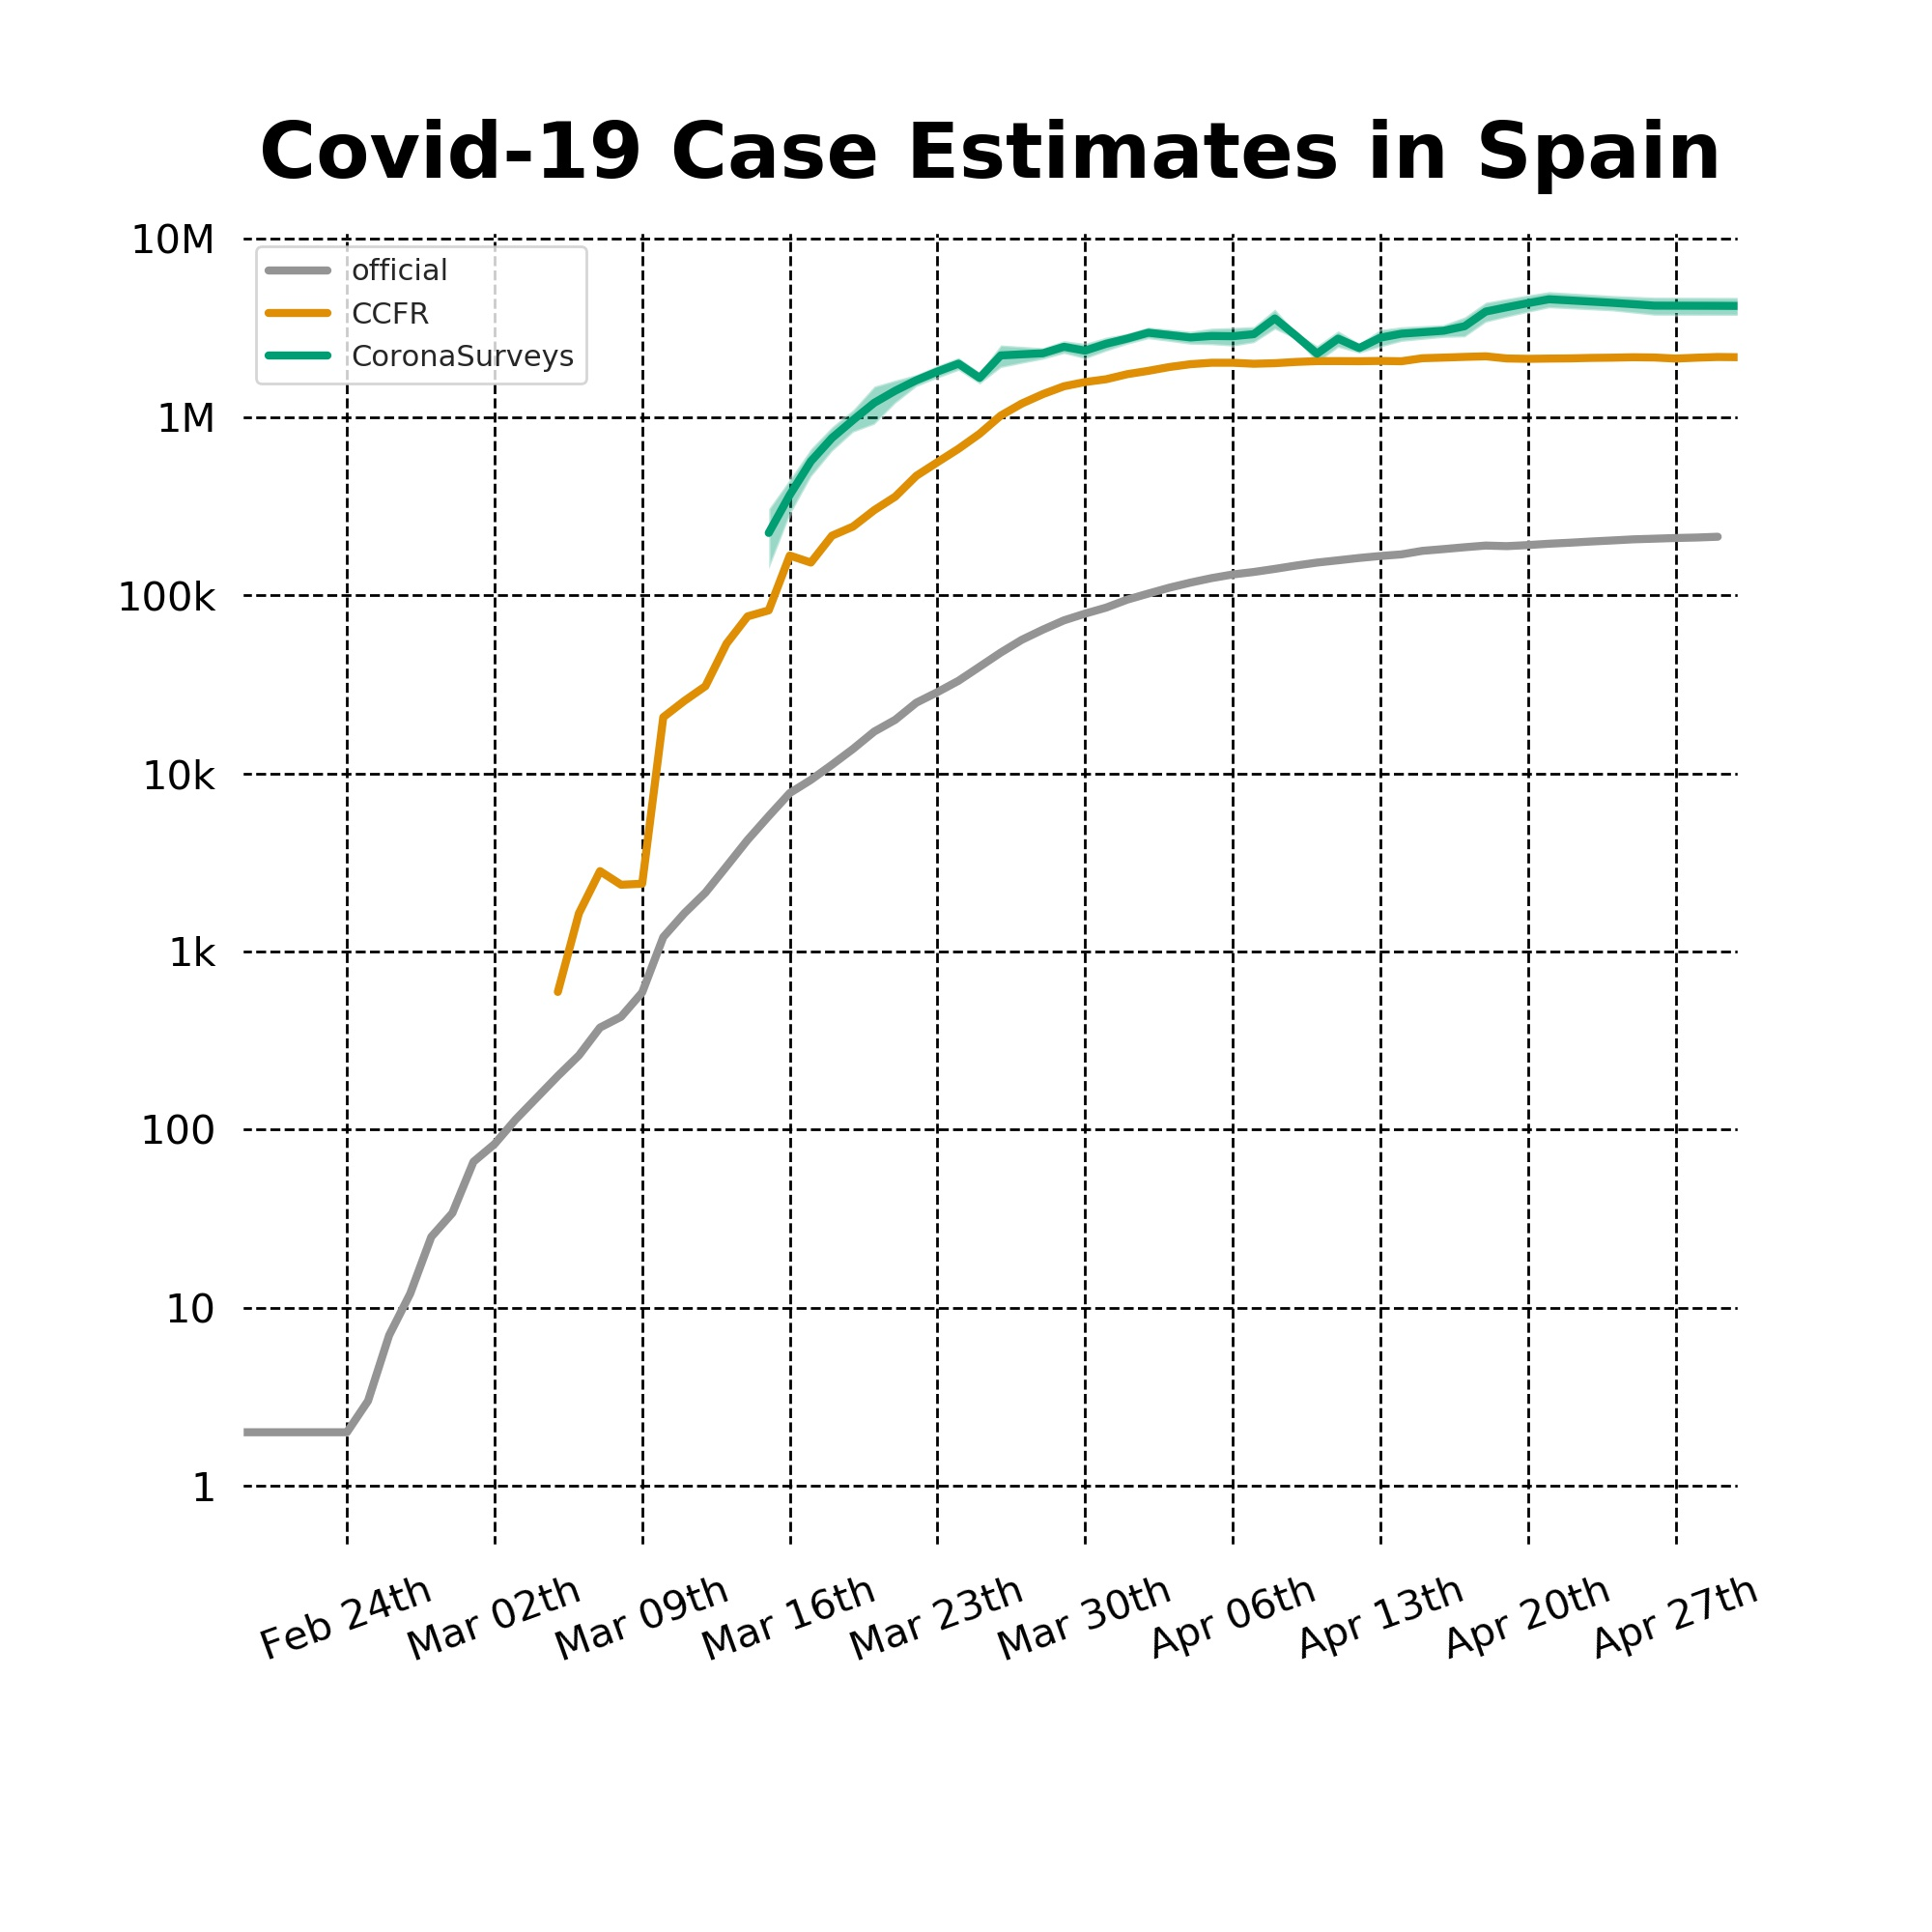
\includegraphics[width=0.7\textwidth]{estimatesES.jpg}
  \end{center}
\end{frame}

\begin{frame}
  \frametitle{Estimates, France}
  \begin{center}
  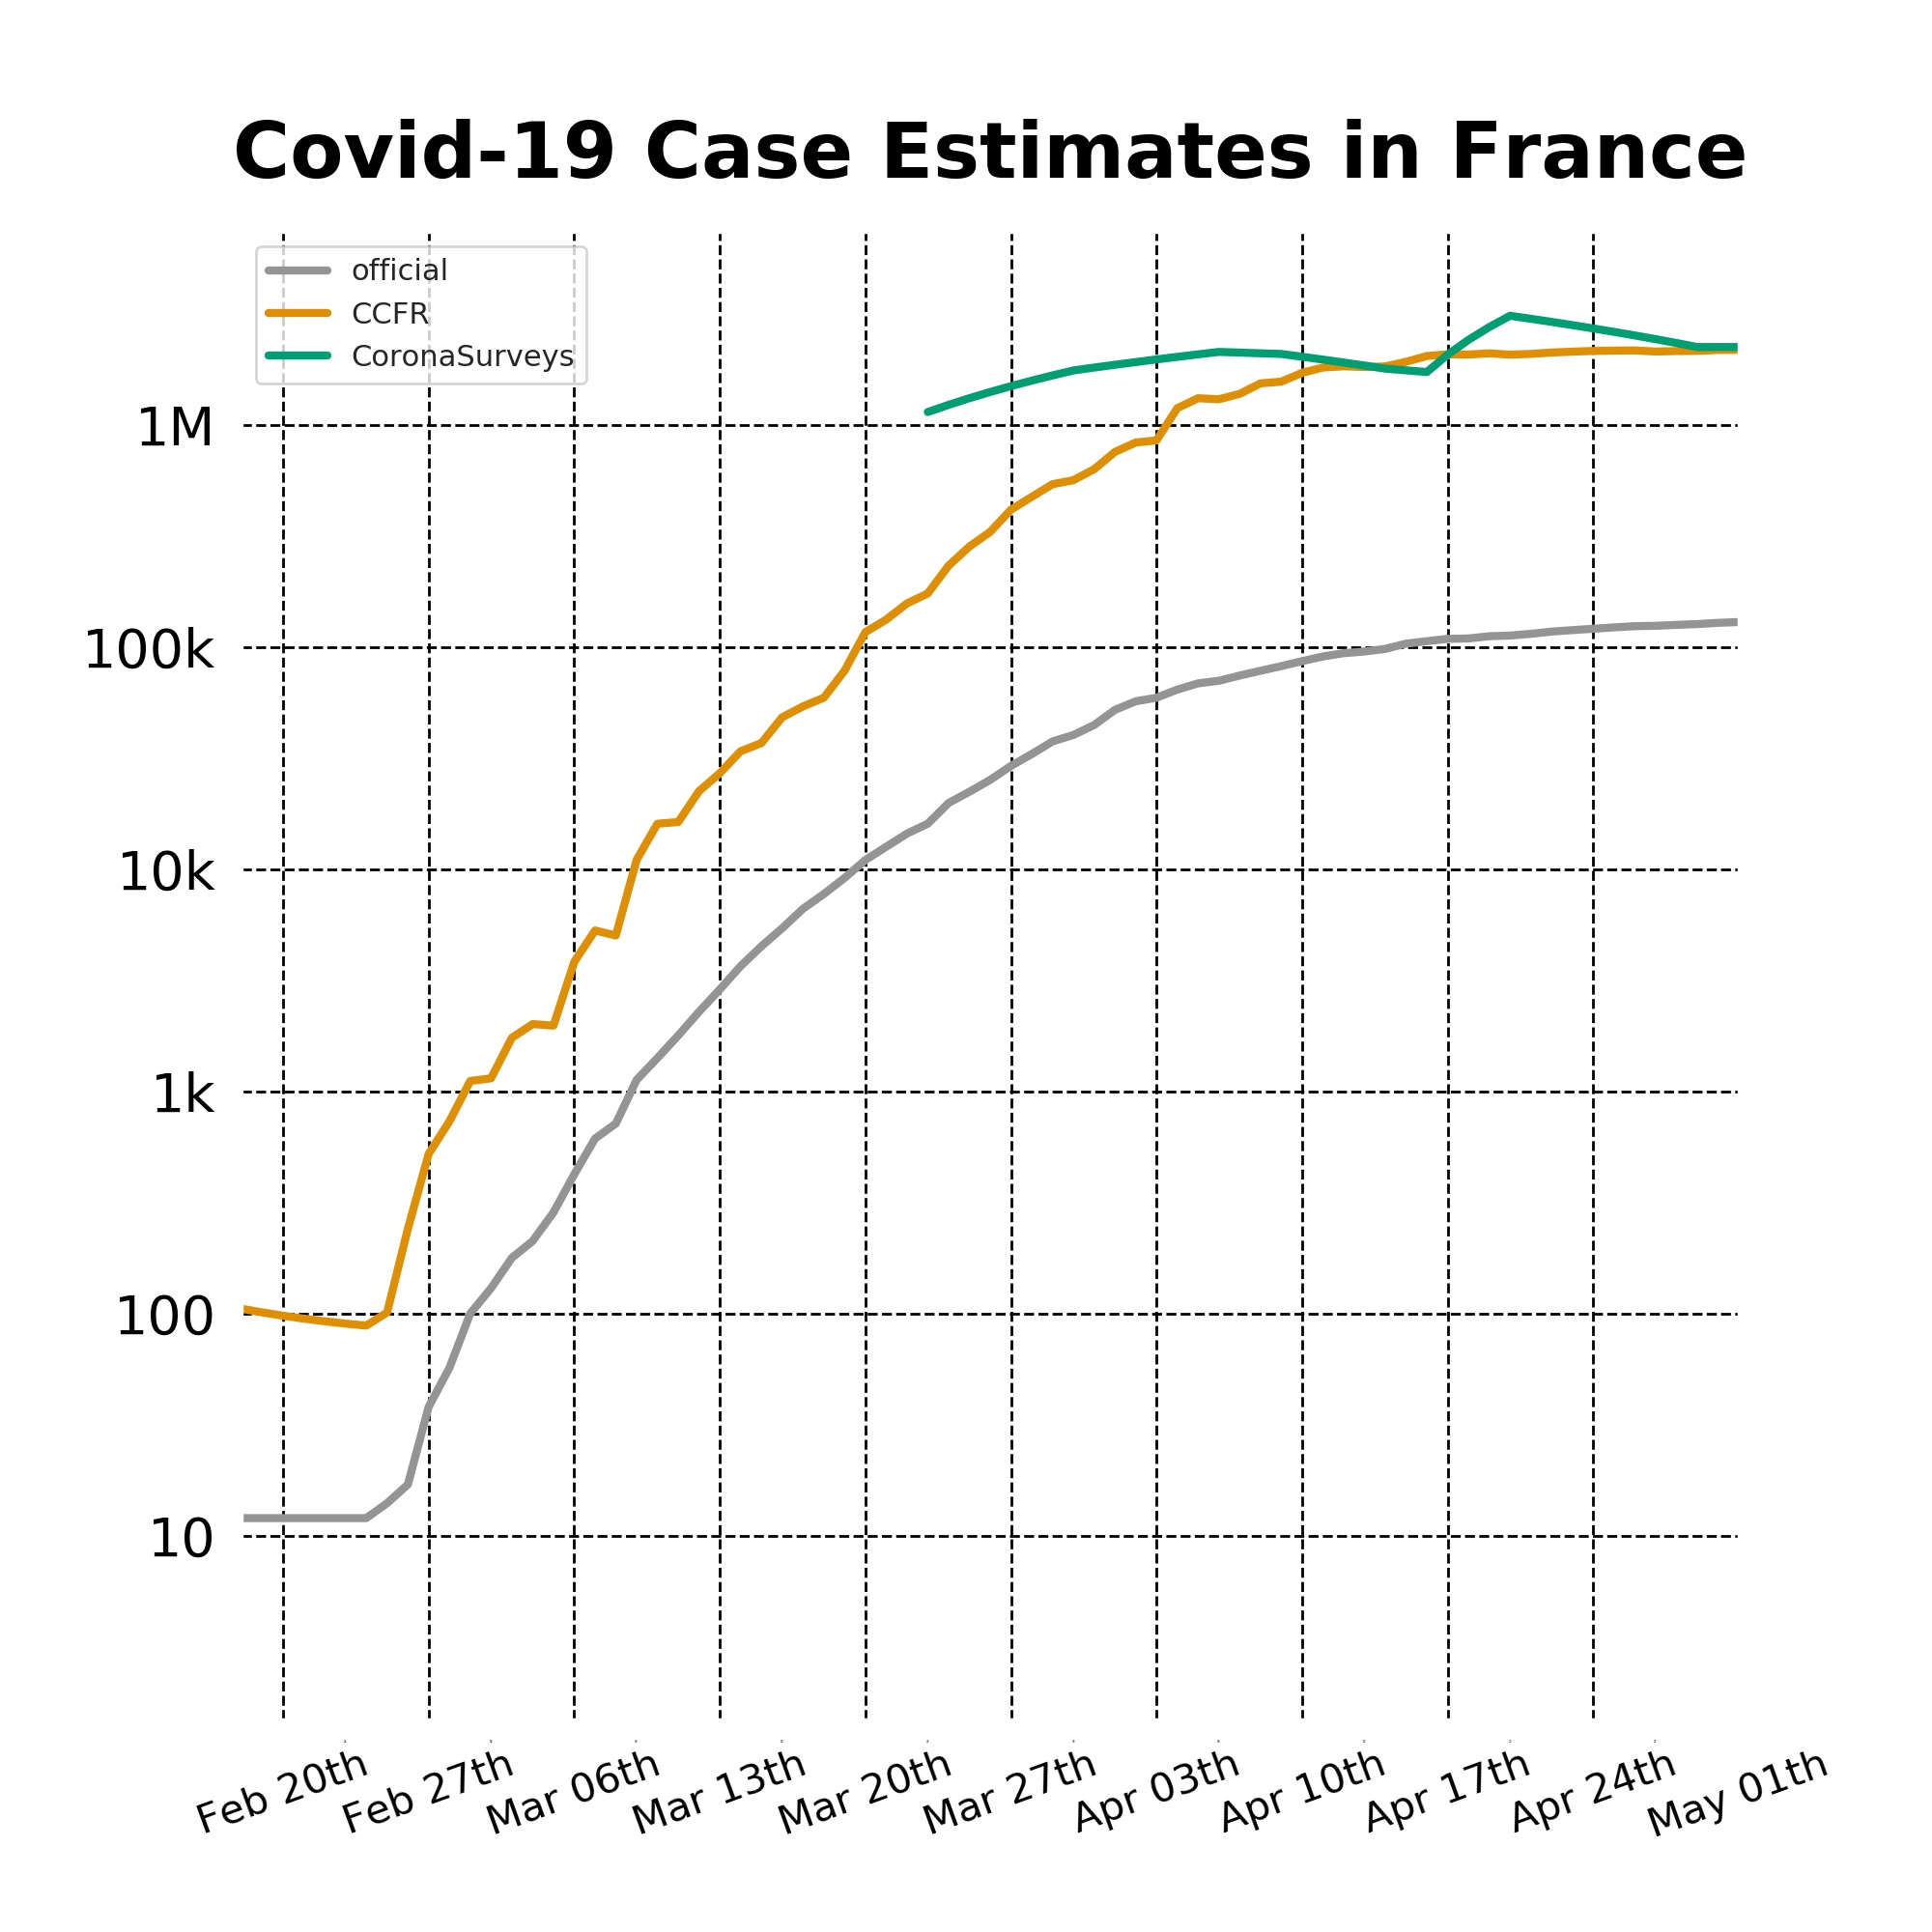
\includegraphics[width=0.7\textwidth]{estimatesFR.jpg}
  \end{center}
\end{frame}

\begin{frame}
  \frametitle{@Coronasurveys, status and potential uses}
  \begin{itemize}
    \item Data is being collected since mid March
    \item We are calibrating as the pandemic and data evolves
    \item Surveys are open for all globe
    \item New regional-based estimates
    \item Survey improvements to reduce bias
  \end{itemize}
  \begin{itemize}
    \item Potential for quick assessment when reliable techniques lack 
    \item Countries with good digital penetration but lacking testing
  \end{itemize}

\end{frame}

\begin{frame}
  \frametitle{Portfolio}
  \framesubtitle{Countries}
  \begin{center}
  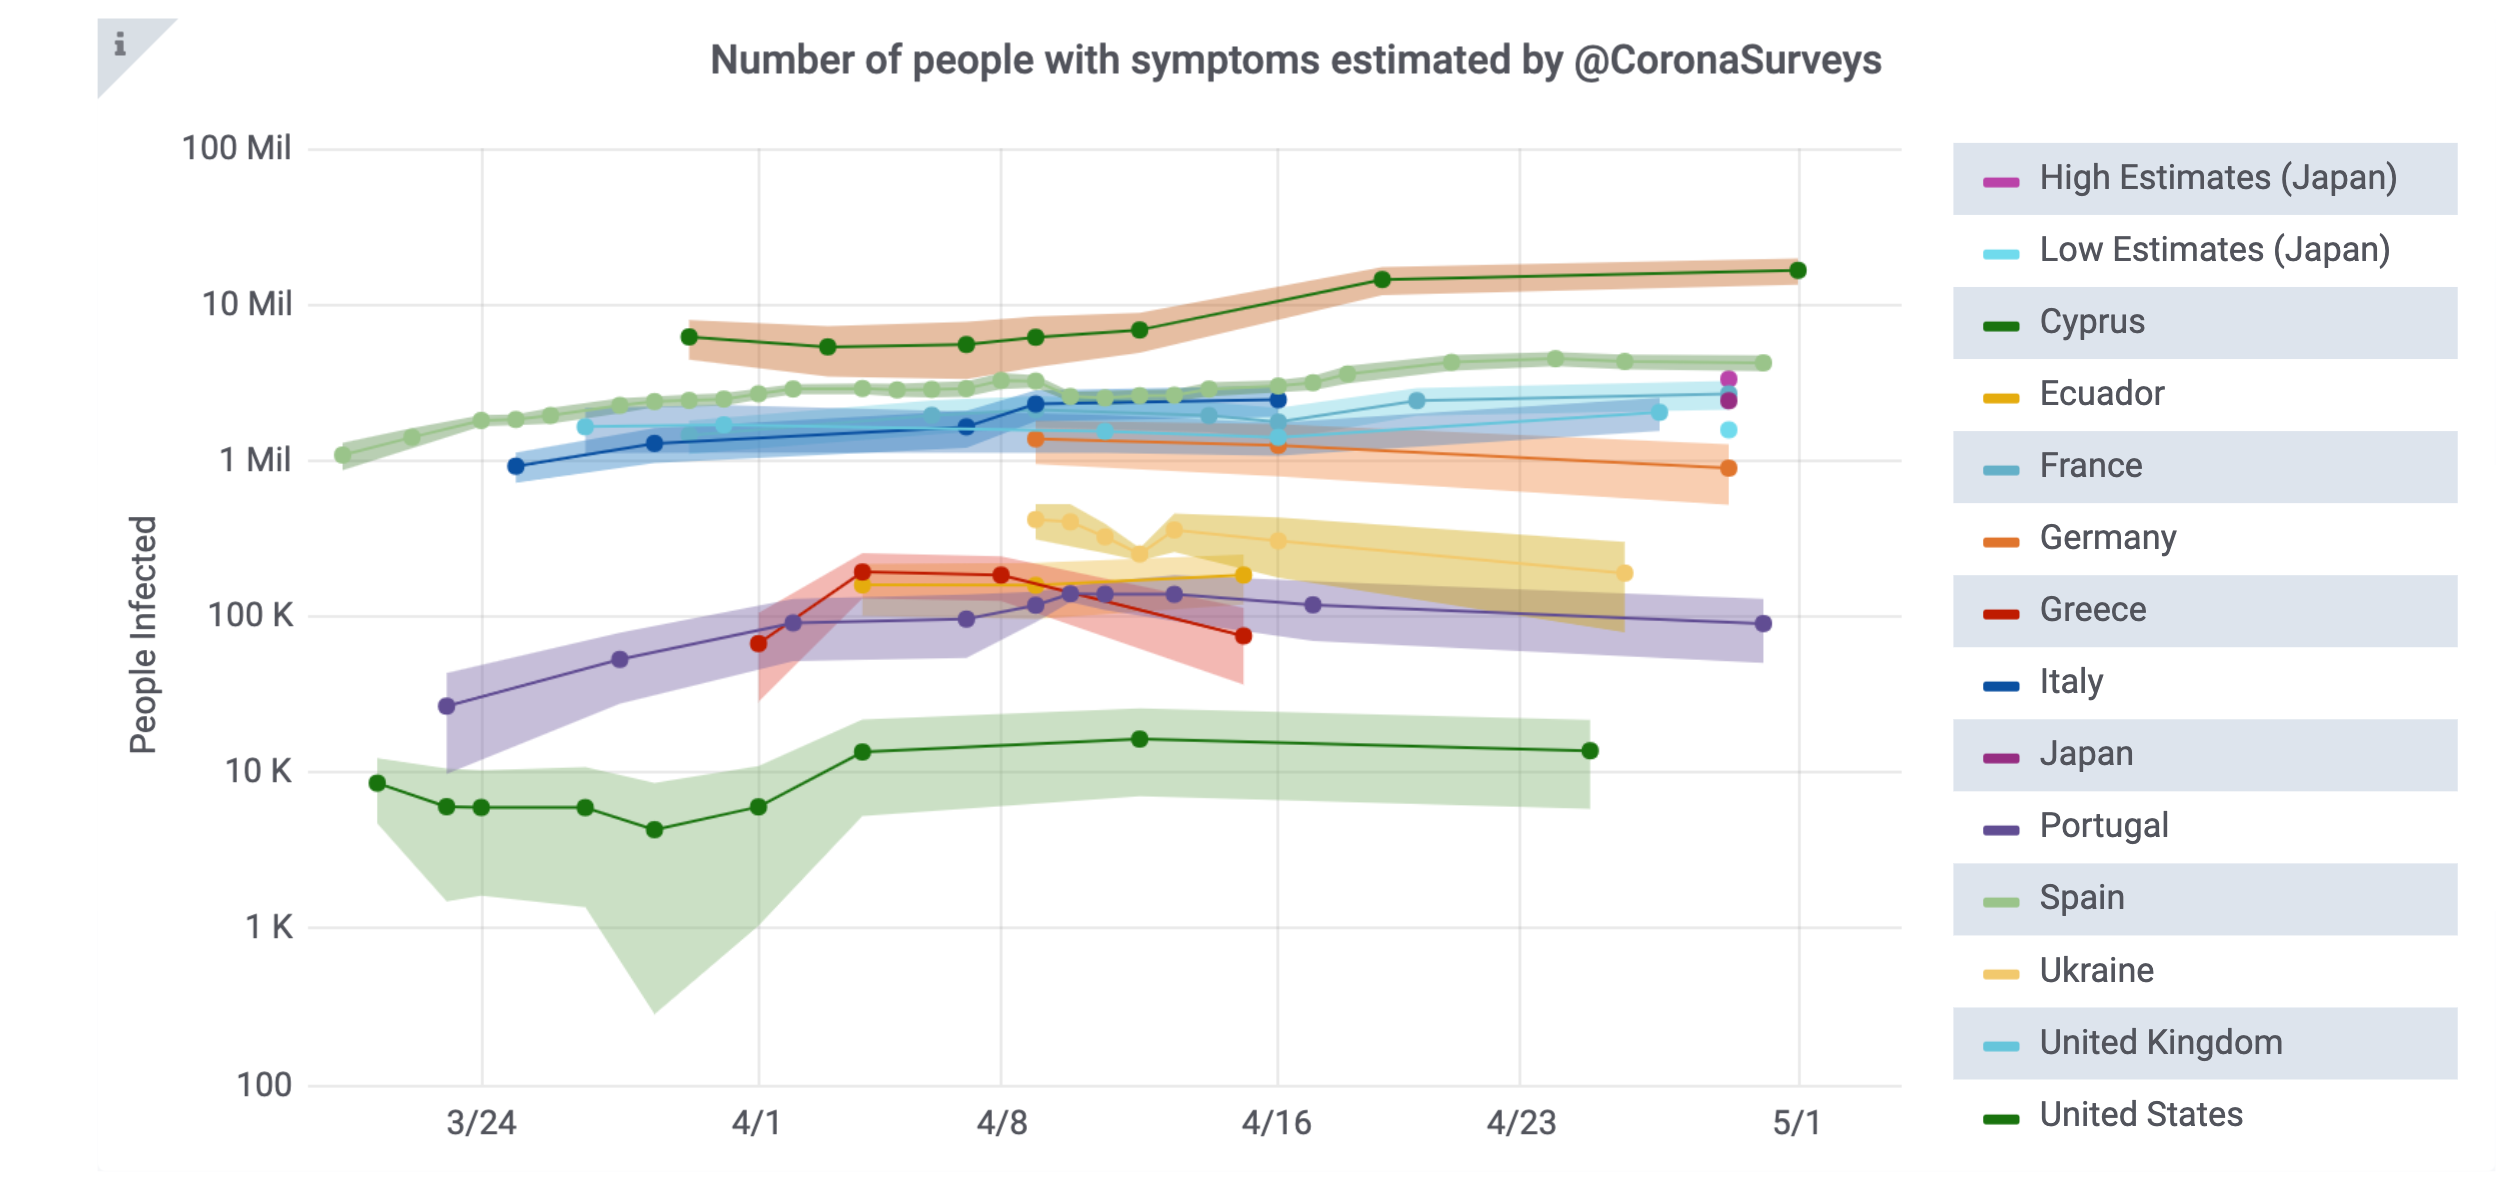
\includegraphics[width=0.9\textwidth]{allcountries.png}
  \end{center}
\end{frame}

% \begin{frame}
%   \frametitle{Portfolio}
%   \framesubtitle{France}
%   \begin{center}
%   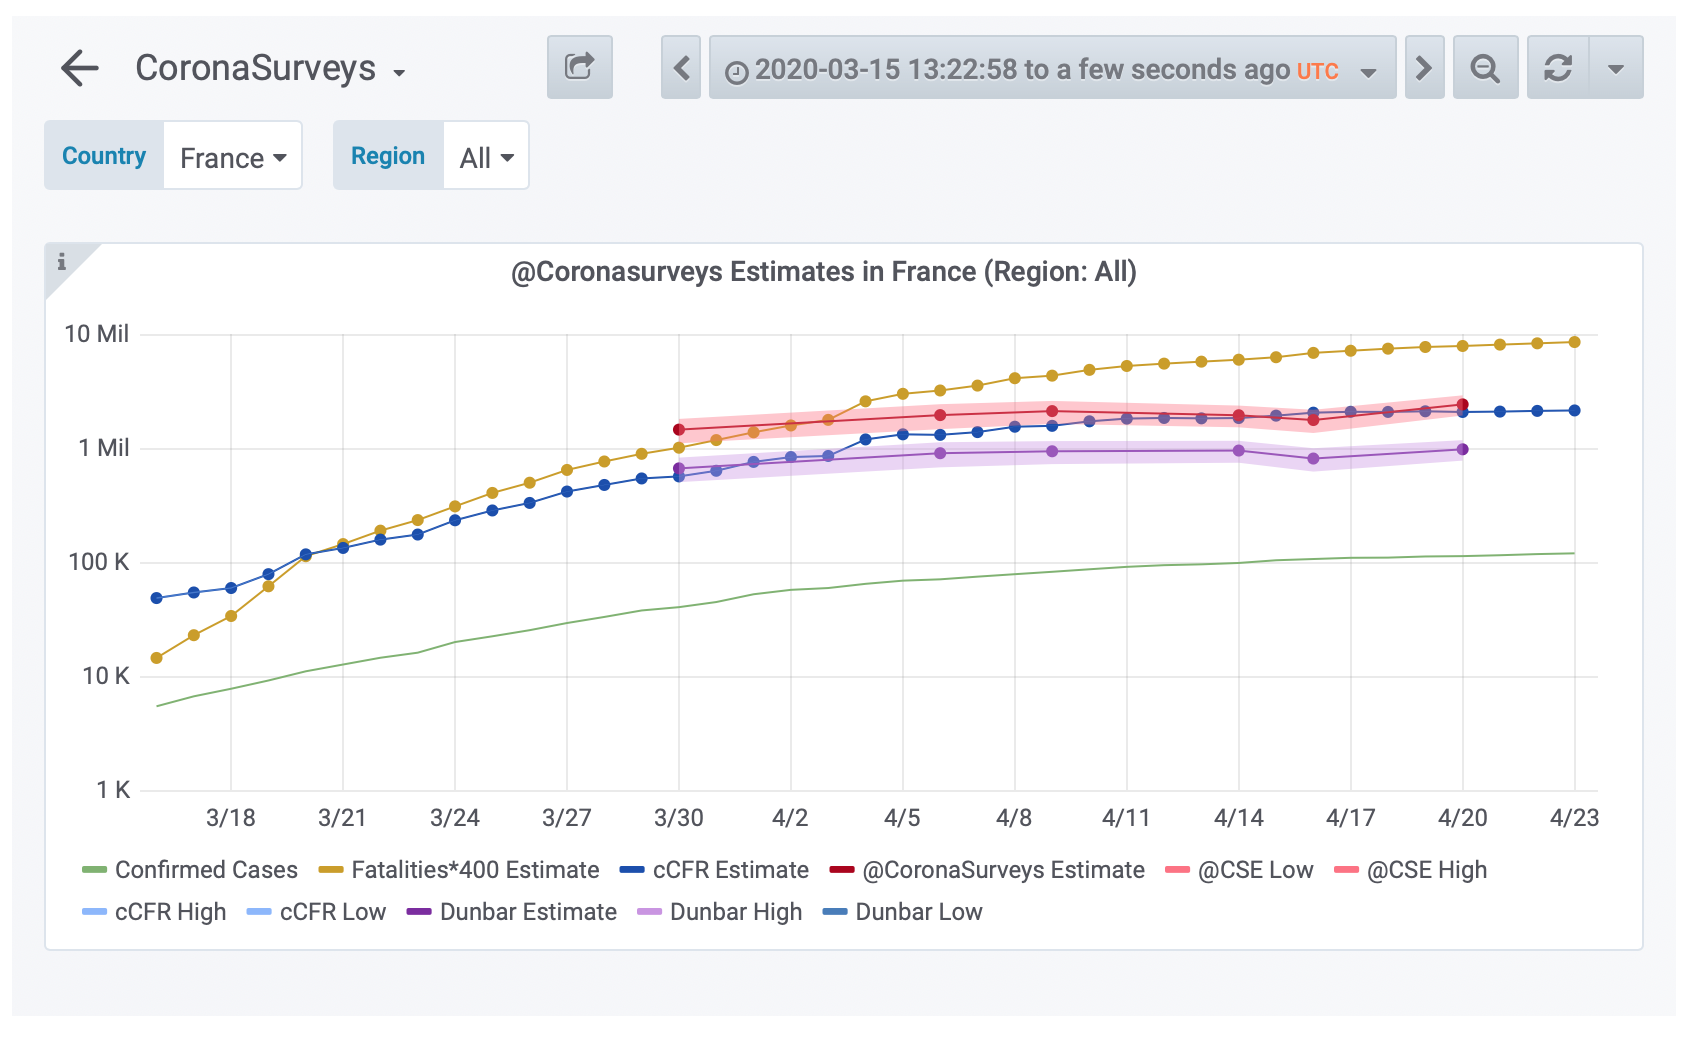
\includegraphics[width=0.9\textwidth]{France.png}
%   \end{center}
% \end{frame}

% \begin{frame}
%   \frametitle{Portfolio}
%   \framesubtitle{Australia}
%   \begin{center}
%   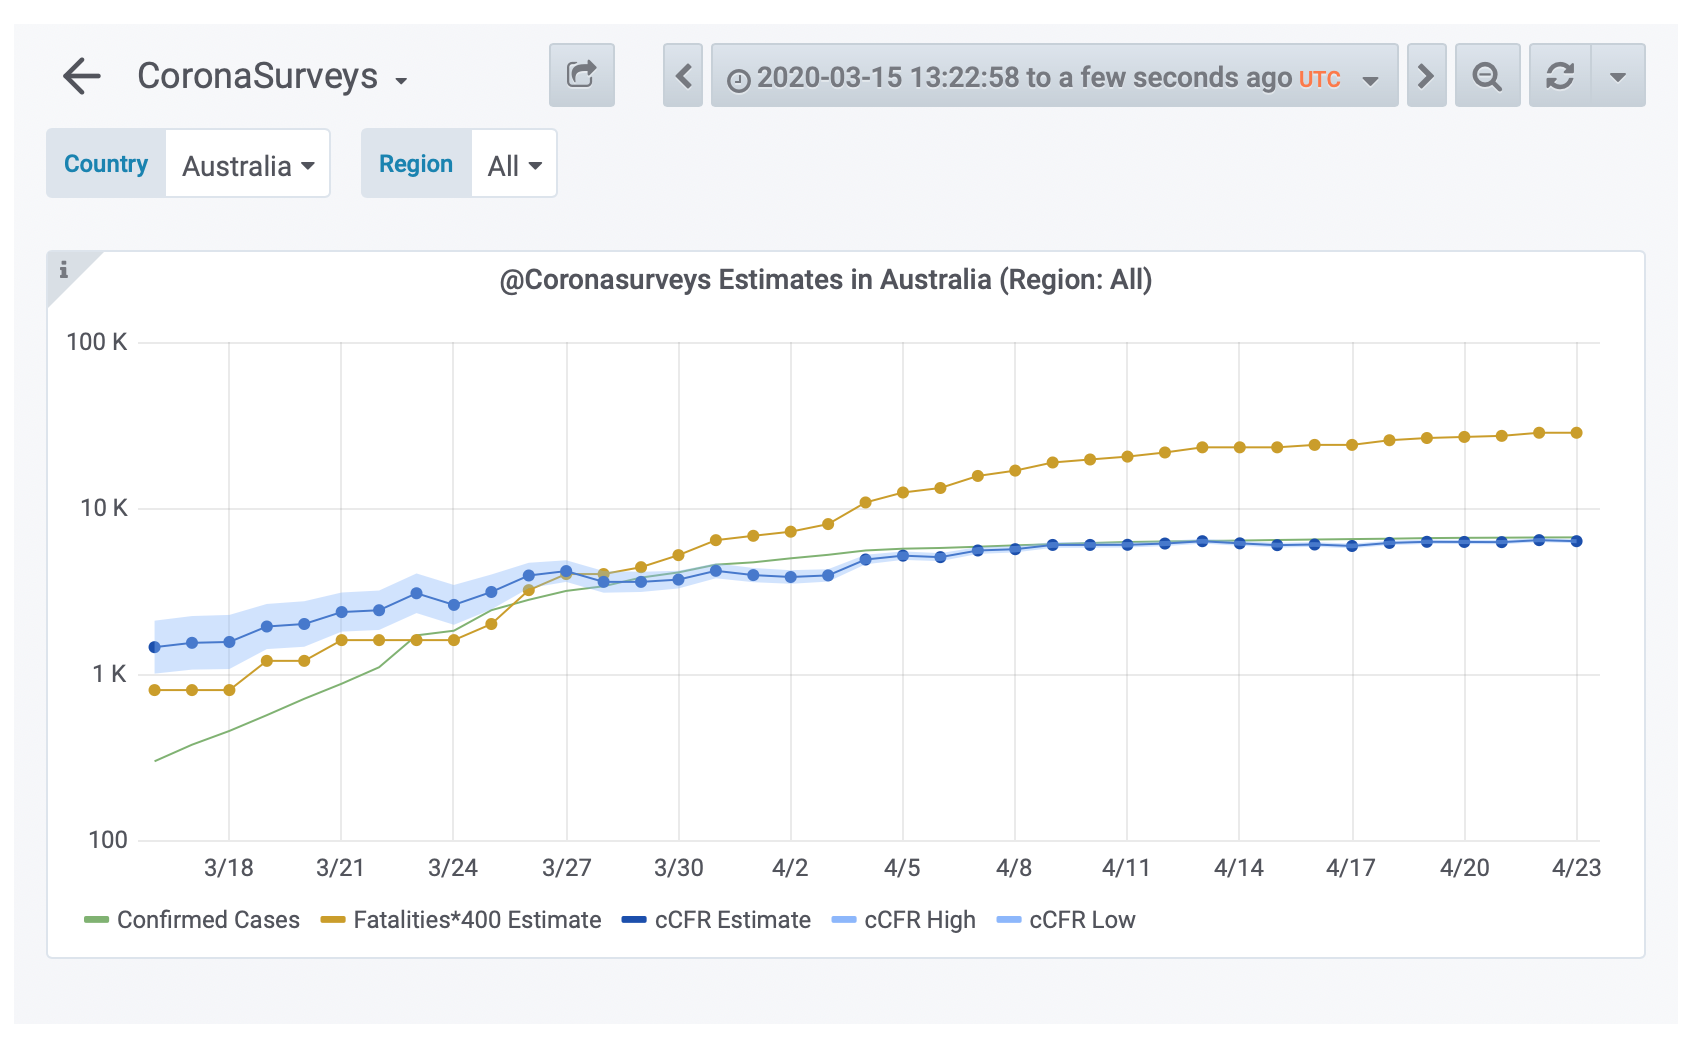
\includegraphics[width=0.9\textwidth]{Australia.png}
%   \end{center}
%   Closely matching Wuhan baseline
% \end{frame}

% \begin{frame}
%   \frametitle{Portfolio}
%   \framesubtitle{Portugal}
%   \begin{center}
%   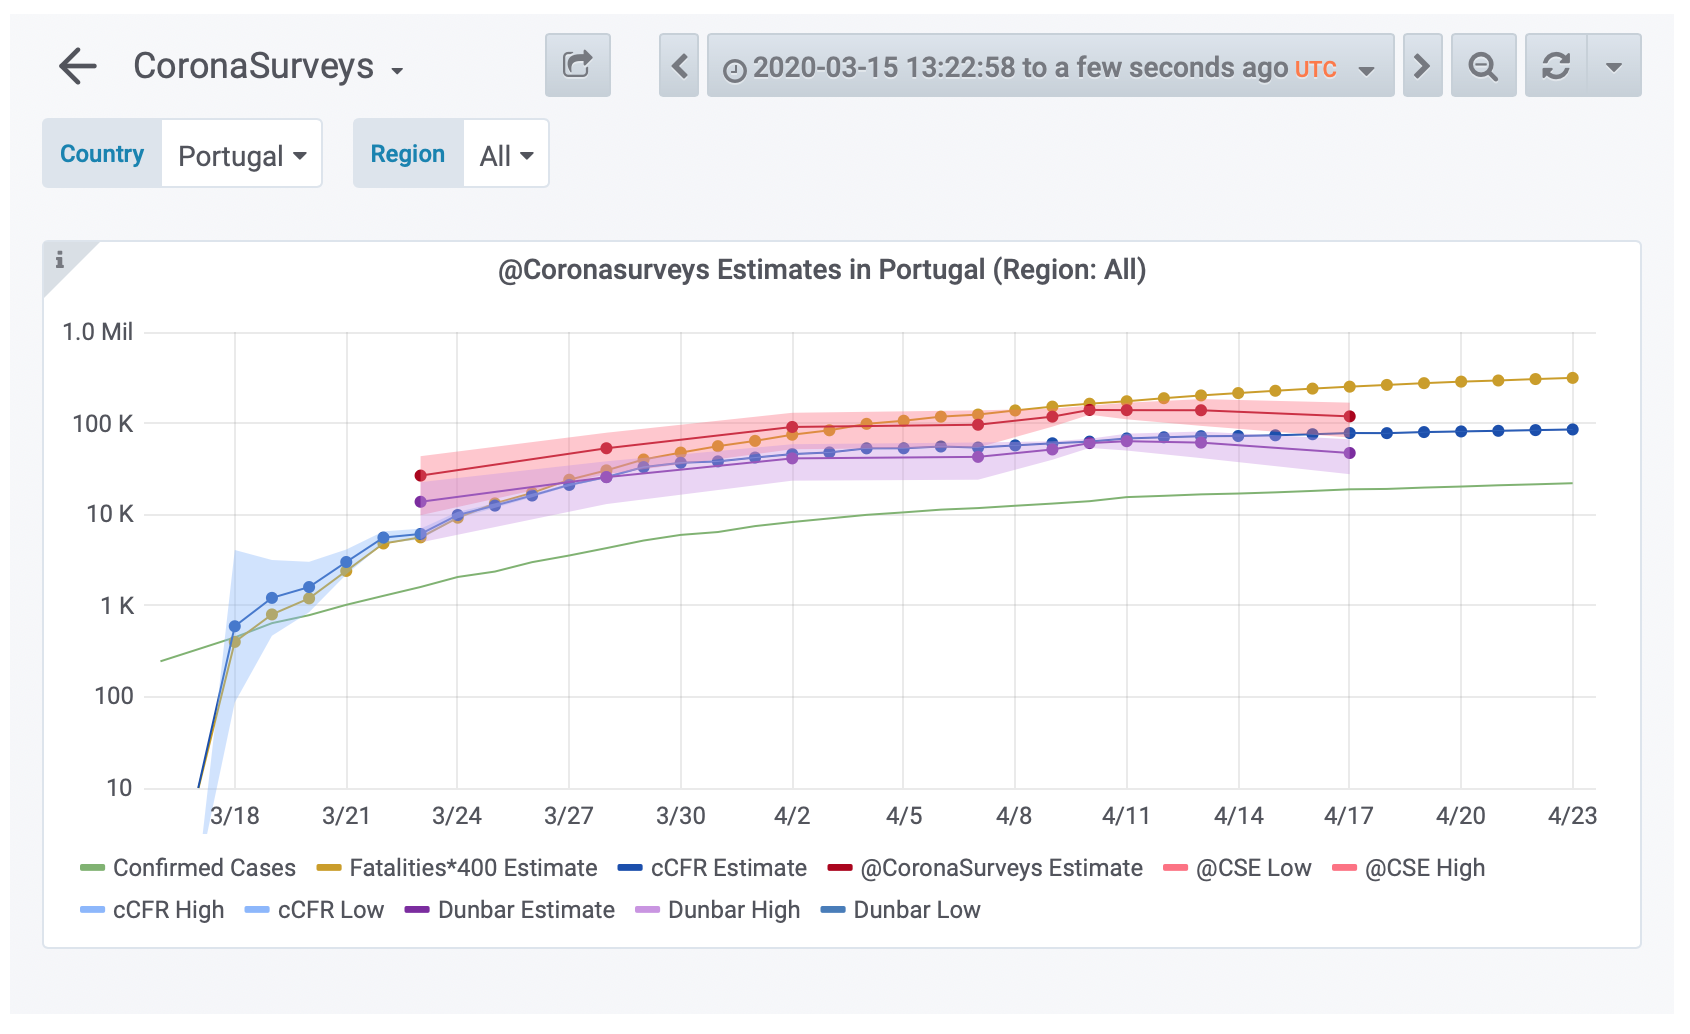
\includegraphics[width=0.9\textwidth]{Portugal.png}
%   \end{center}
% \end{frame}

% \begin{frame}
%   \frametitle{Portfolio}
%   \framesubtitle{Portugal ARS Norte}
%   \begin{center}
%   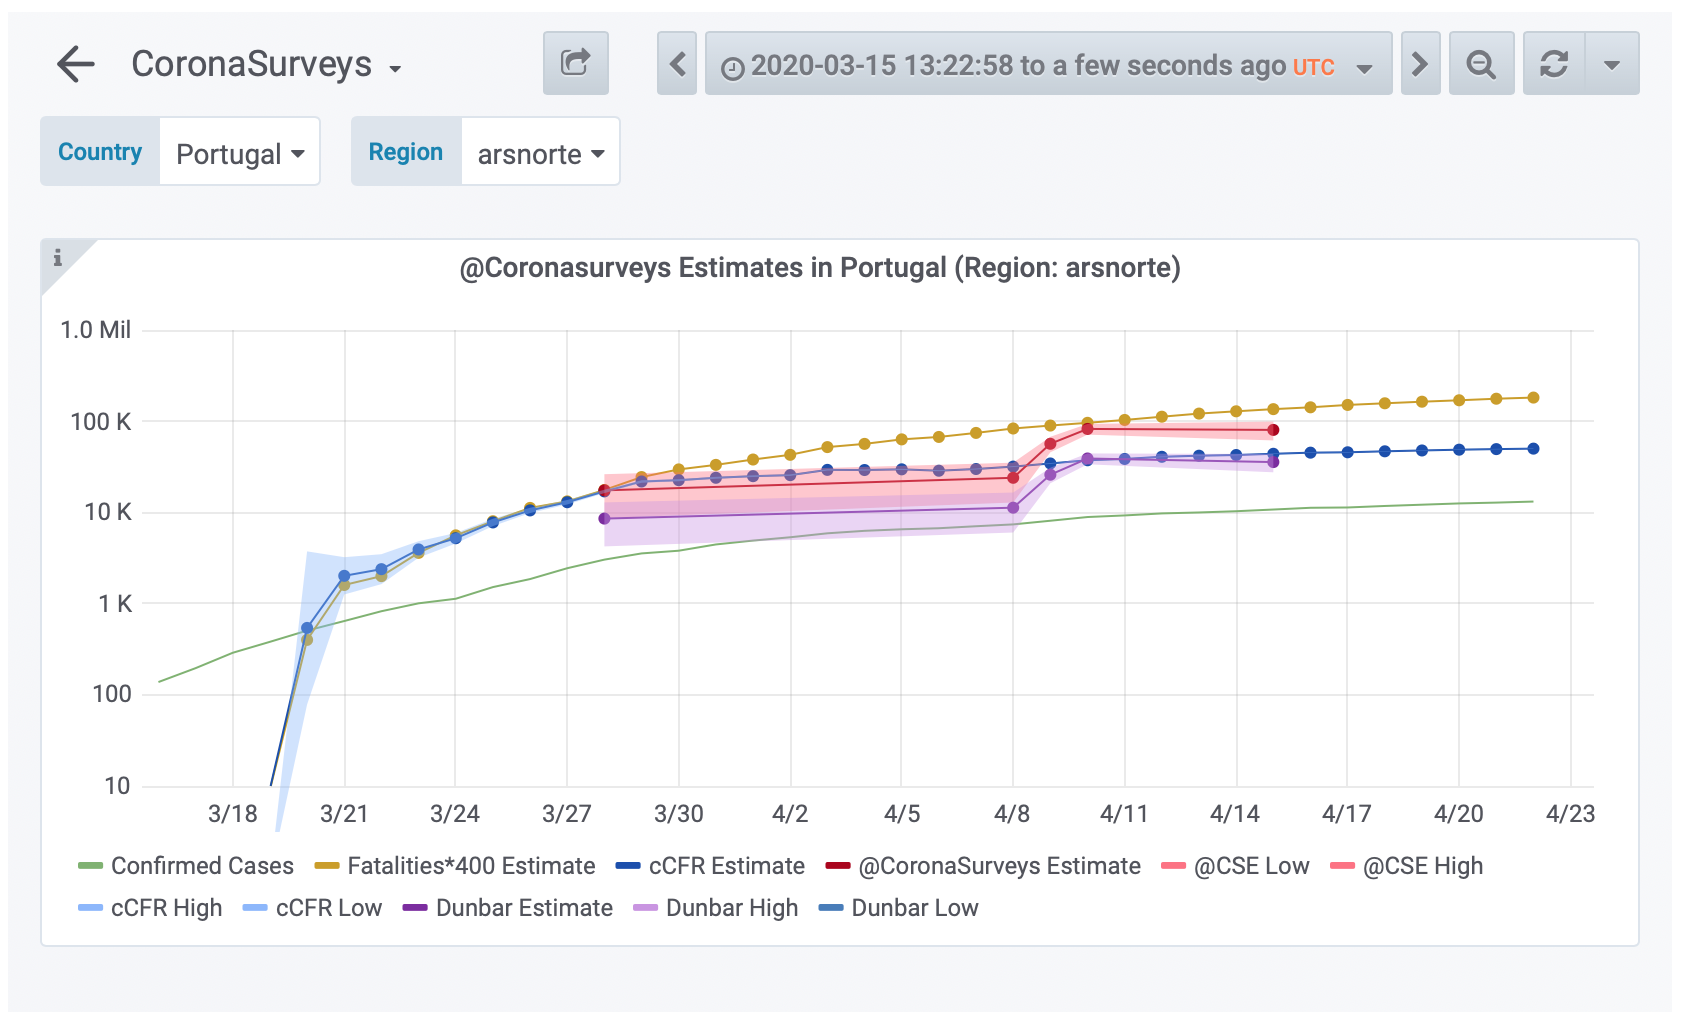
\includegraphics[width=0.9\textwidth]{PortugalNorte.png}
%   \end{center}
%   Data by regions in some countries
% \end{frame}

% \begin{frame}
%   \frametitle{Portfolio}
%   \framesubtitle{Cyprus}
%   \begin{center}
%   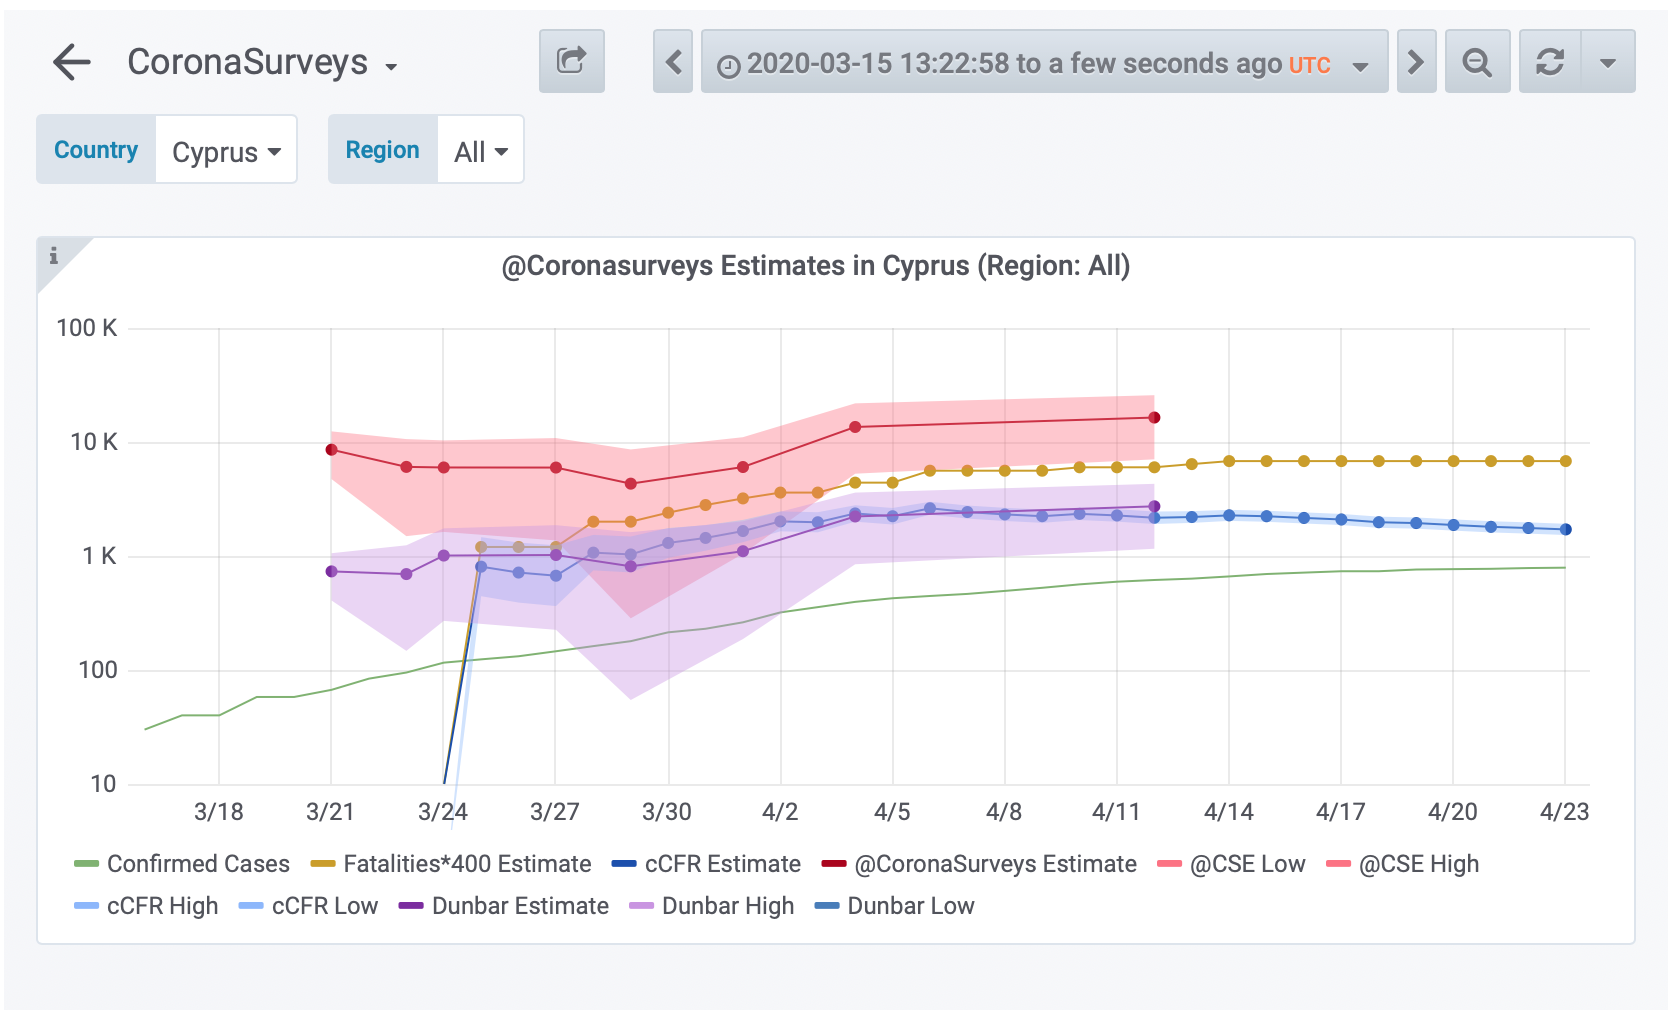
\includegraphics[width=0.9\textwidth]{Cyprus.png}
%   \end{center}
%   Survey estimates preceded fatalities derived estimates
% \end{frame}

% \begin{frame}
%   \frametitle{Portfolio}
%   \framesubtitle{Ukraine}
%   \begin{center}
%   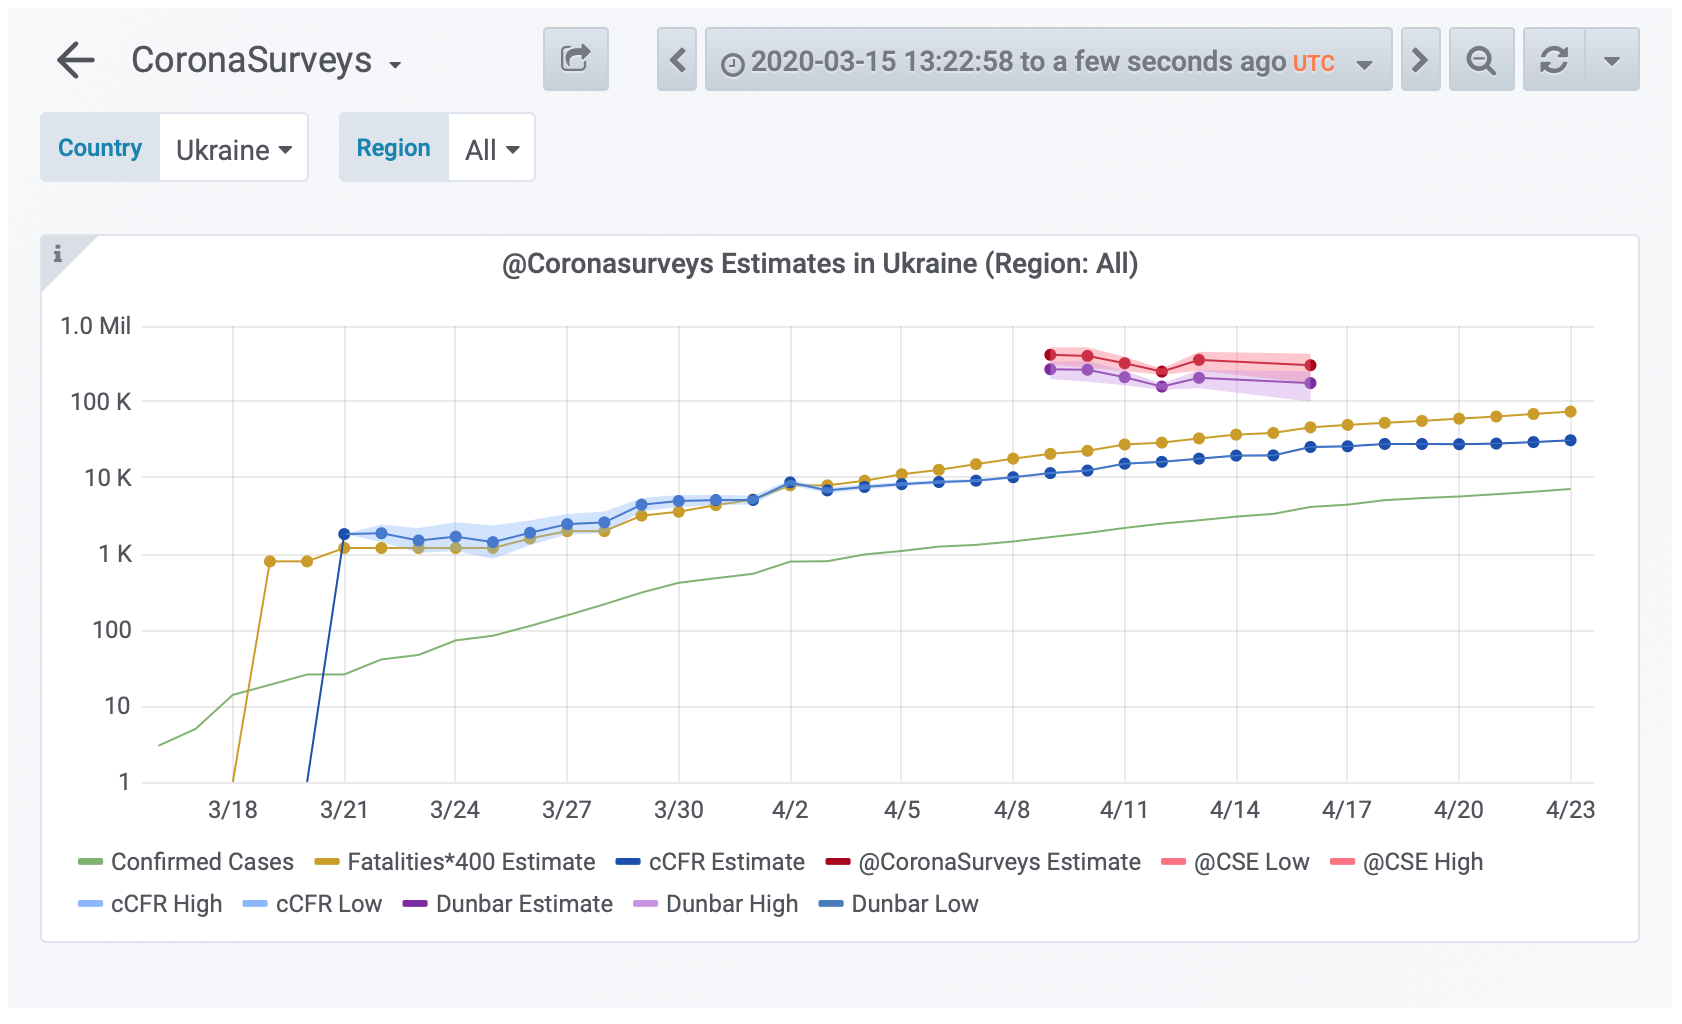
\includegraphics[width=0.9\textwidth]{Ukraine.png}
%   \end{center}
%   Potential under-reporting of deaths
% \end{frame}




\begin{frame}
  \frametitle{Questions?}
  \framesubtitle{@CoronaSurveys at http://coronasurveys.org}
  \begin{center}
  
\includegraphics[width=0.3\textwidth]{CoronaSurveys.png}
  \end{center}
  \begin{itemize}
    \item
  https://www.instagram.com/coronasurveys/
  \item
  https://tinyurl.com/coronasurveysfrance
\item
  Twitter: @coronasurveys
\item
  https://www.instagram.com/coronasurveys/ 
\item
  FB: https://www.facebook.com/groups/209076966867175

  \vspace{1ex}
\item
  Both our raw and processed data is openly available
  https://github.com/GCGImdea/coronasurveys
\end{itemize}
\end{frame}


\end{document}
